% !TEX encoding = UTF-8 Unicode
\documentclass{wissdoc}
% Autor: Chi Trung Nguyen 2013-2014, chitrungnguyen <at> me.com
% Vorlagenautor: Roland Bless 1996-2009, bless <at> kit.edu
% ----------------------------------------------------------------
% Diplomarbeit - Hauptdokument
% ----------------------------------------------------------------
%%
%% $Id: thesis.tex 65 2012-05-10 10:32:11Z bless $
%%
% wissdoc Optionen: draft, relaxed, pdf --> siehe wissdoc.cls
% ------------------------------------------------------------------
% Weitere packages: (Dokumentation dazu durch "latex <package>.dtx")
\usepackage[numbers,sort&compress]{natbib}
\usepackage{float}
\restylefloat{table} %!damit tabellen dort auftauchen, wo sie beschrieben werden([H] benutzen!)
\usepackage[official]{eurosym} % für Eurosymbol
%\usepackage{listings} %für Quellcode
% \lstset{
%   literate={Ö}{{\"O}}1
% {Ä}{{\"A}}1
% {Ü}{{\"U}}1
% {ß}{{\ss}}2
% {Ì}{{\"u}}1
% {À}{{\"a}}1
% {ö}{{\"o}}1
% }
% \usepackage{varioref}
% \usepackage{verbatim}
% \usepackage{float}    %z.B. \floatstyle{ruled}\restylefloat{figure}
% \usepackage{subfigure}
% \usepackage{fancybox} % fÃŒr schattierte,ovale Boxen etc.
% \usepackage{tabularx} % automatische Spaltenbreite
% \usepackage{supertab} % mehrseitige Tabellen
% \usepackage[svnon,svnfoot]{svnver} % SVN Versionsinformation 
%% ---------------- end of usepackages -------------

%\svnversion{$Id: thesis.tex 65 2012-05-10 10:32:11Z bless $} % In case that you want to include version information in the footer

%% Informationen fÃŒr die PDF-Datei
\hypersetup{
 pdfauthor={Andreas Hornig, Florian Weber, Chi Trung Nguyen},
 pdftitle={Not set}
 pdfsubject={Not set},
 pdfkeywords={Not set}
}

% Macros, nicht unbedingt notwendig
%%%%%%%%%%%%%%%%%%%%%%%%%%%%%%%%%%%%%%%%%%%%%%%%%%%%%%%%%%
% macros.tex -- einige mehr oder weniger nuetzliche Makros
% Autor: Roland Bless 1998
%%%%%%%%%%%%%%%%%%%%%%%%%%%%%%%%%%%%%%%%%%%%%%%%%%%%%%%%%%
% $Id: macros.tex 33 2007-01-23 09:00:59Z bless $
%%%%%%%%%%%%%%%%%%%%%%%%%%%%%%%%%%%%%%%%%%%%%%%%%%%%%%%%%%


%%%%%%%%%%%%%%%%%%%%%%%
% Kommentare 
%%%%%%%%%%%%%%%%%%%%%%%
\ifnotdraftelse{
\newcommand{\Kommentar}[1]{}
}{\newcommand{\Kommentar}[1]{{\em #1}}}
% Alles innerhalb von \Hide{} oder \ignore{} 
% wird von LaTeX komplett ignoriert (wie ein Kommentar)
\newcommand{\Hide}[1]{}
\let\ignore\Hide

%%%%%%%%%%%%%%%%%%%%%%%%%
% Leere Seite ohne Seitennummer, wird aber gezaehlt
%%%%%%%%%%%%%%%%%%%%%%%%%

\newcommand{\leereseite}{% Leerseite ohne Seitennummer, nächste Seite rechts (wenn 2-seitig)
 \clearpage{\pagestyle{empty}\cleardoublepage}
}
%%%%%%%%%%%%%%%%%%%%%%%%%%
% Flattersatz rechts und Silbentrennung, Leerraum nach rechts maximal 1cm
%%%%%%%%%%%%%%%%%%%%%%%%%%
\makeatletter
\newcommand{\myraggedright}{%
 \let\\\@centercr\@rightskip 0pt plus 1cm
 \rightskip\@rightskip
  \leftskip\z@skip
  \parindent\z@
  \spaceskip=.3333em
  \xspaceskip=.5em}
\makeatother

\makeatletter
\newcommand{\mynewline}{%
 \@centercr\@rightskip 0pt plus 1cm
}
\makeatother


%%%%%%%%%%%%%%%%%%%%%%%%%%
% Für Index
%%%%%%%%%%%%%%%%%%%%%%%%%%
\makeatletter
\def\mydotfill{\leavevmode\xleaders\hb@xt@ .44em{\hss.\hss}\hfill\kern\z@}
\makeatother
\def\bold#1{{\bfseries #1}}
\newbox\dbox \setbox\dbox=\hbox to .4em{\hss.\hss} % dot box for leaders
\newskip\rrskipb \rrskipb=.5em plus3em % ragged right space before break
\newskip\rrskipa \rrskipa=-.17em plus -3em minus.11em % ditto, after
\newskip\rlskipa \rlskipa=0pt plus3em % ragged left space after break
\newskip\rlskipb \rlskipb=.33em plus-3em minus.11em % ragged left before break
\newskip\lskip \lskip=3.3\wd\dbox plus1fil minus.3\wd\dbox % for leaders
\newskip \lskipa \lskipa=-2.67em plus -3em minus.11em %after leaders
\mathchardef\rlpen=1000 \mathchardef\leadpen=600
\def\rrspace{\nobreak\hskip\rrskipb\penalty0\hskip\rrskipa}
\def\rlspace{\penalty\rlpen\hskip\rlskipb\vadjust{}\nobreak\hskip\rlskipa}
\let\indexbreak\rlspace
\def\raggedurl{\penalty10000 \hskip.5em plus15em \penalty0 \hskip-.17em plus-15em minus.11em}
\def\raggeditems{\nobreak\hskip\rrskipb \penalty\leadpen \hskip\rrskipa %
\vadjust{}\nobreak\leaders\copy\dbox\hskip\lskip %
\kern3em \penalty\leadpen \hskip\lskipa %
\vadjust{}\nobreak\hskip\rlskipa}
\renewcommand*\see[2]{\rlspace\emph{\seename}~#1} % from makeidx.sty

%%%%%%%%%%%%%%%%%%%%%%%%%%
% Neue Seite rechts, leere linke Seite ohne Headings
%%%%%%%%%%%%%%%%%%%%%%%%%%
\newcommand{\xcleardoublepage}
{{\pagestyle{empty}\cleardoublepage}}

%%%%%%%%%%%%%%%%%%%%%%%%%%
% Tabellenspaltentypen (benoetigt colortbl)
%%%%%%%%%%%%%%%%%%%%%%%%%%
\newcommand{\PBS}[1]{\let\temp=\\#1\let\\=\temp}
\newcolumntype{y}{>{\PBS{\raggedright\hspace{0pt}}}p{1.35cm}}
\newcolumntype{z}{>{\PBS{\raggedright\hspace{0pt}}}p{2.5cm}}
\newcolumntype{q}{>{\PBS{\raggedright\hspace{0pt}}}p{6.5cm}}
\newcolumntype{g}{>{\columncolor[gray]{0.8}}c} % Grau
\newcolumntype{G}{>{\columncolor[gray]{0.9}}c} % helleres Grau

%%%%%%%%%%%%%%%%%%%%%%%%%%
% Anführungszeichen oben und unten
%%%%%%%%%%%%%%%%%%%%%%%%%%
\newcommand{\anf}[1]{"`{#1}"'}

%%%%%%%%%%%%%%%%%%%%%%%%%%
% Tiefstellen von Text
%%%%%%%%%%%%%%%%%%%%%%%%%%
% S\tl{0} setzt die 0 unter das S (ohne Mathemodus!)
% zum Hochstellen gibt es uebrigens \textsuperscript
\makeatletter
\DeclareRobustCommand*\textlowerscript[1]{%
  \@textlowerscript{\selectfont#1}}
\def\@textlowerscript#1{%
  {\m@th\ensuremath{_{\mbox{\fontsize\sf@size\z@#1}}}}}
\let\tl\textlowerscript
\let\ts\textsuperscript
\makeatother

%%%%%%%%%%%%%%%%%%%%%%%%%%
% Gauß-Klammern
%%%%%%%%%%%%%%%%%%%%%%%%%%
\newcommand{\ceil}[1]{\lceil{#1}\rceil}
\newcommand{\floor}[1]{\lfloor{#1}\rfloor}

%%%%%%%%%%%%%%%%%%%%%%%%%%
% Average Operator (analog zu min, max)
%%%%%%%%%%%%%%%%%%%%%%%%%%
\def\avg{\mathop{\mathgroup\symoperators avg}}

%%%%%%%%%%%%%%%%%%%%%%%%%%
% Wortabkürzungen
%%%%%%%%%%%%%%%%%%%%%%%%%%
\def\zB{z.\,B.\ }
\def\dh{d.\,h.\ }
\def\ua{u.\,a.\ }
\def\su{s.\,u.\ }
\newcommand{\bzw}{bzw.\ }

%%%%%%%%%%%%%%%%%%%%%%%%%%%%%%%%%%%
% Einbinden von Graphiken
%%%%%%%%%%%%%%%%%%%%%%%%%%%%%%%%%%%
% global scaling factor
\def\gsf{0.9}
%% Graphik, 
%% 3 Argumente: Datei, Label, Unterschrift
\newcommand{\Abbildung}[3]{%
\begin{figure}[tbh] %
\centerline{\scalebox{\gsf}{\includegraphics*{#1}}} %
\caption{#3} %
\label{#2} %
\end{figure} %
}
\let\Abb\Abbildung
%% Abbps
%% Graphik, skaliert, Angabe der Position
%% 5 Argumente: Position, Breite (0 bis 1.0), Datei, Label, Unterschrift
\newcommand{\Abbildungps}[5]{%
\begin{figure}[#1]%
\begin{center}
\scalebox{\gsf}{\includegraphics*[width=#2\textwidth]{#3}}%
\caption{#5}%
\label{#4}%
\end{center}
\end{figure}%
}
\let\Abbps\Abbildungps
%% Graphik, Angabe der Position, frei wählbares Argument für includegraphics
%% 5 Argumente: Position, Optionen, Datei, Label, Unterschrift
\newcommand{\Abbildungpf}[5]{%
\begin{figure}[#1]%
\begin{center}
\scalebox{\gsf}{\includegraphics*[#2]{#3}}%
\caption{#5}%
\label{#4}%
\end{center}
\end{figure}%
}
\let\Abbpf\Abbildungpf

%%
% Anmerkung: \resizebox{x}{y}{box} skaliert die box auf Breite x und Höhe y,
%            ist x oder y ein !, dann wird das usprüngliche 
%            Seitenverhältnis beibehalten.
%            \rescalebox funktioniert ähnlich, nur das dort ein Faktor
%            statt einer Dimension angegeben wird.
%%
% \Abbps{Position}{Breite in Bruchteilen der Textbreite}{Dateiname}{Label}{Bildunterschrift}
%

\newcommand{\refAbb}[1]{%
s.~Abbildung \ref{#1}}

%%%%%%%%%%%%%%%%%%%%
%% end of macros.tex
%%%%%%%%%%%%%%%%%%%%

% Print URLs not in Typewriter Font
\def\UrlFont{\rm}

\newcommand{\blankpage}{% Leerseite ohne Seitennummer, nÀchste Seite rechts
 \clearpage{\pagestyle{empty}\cleardoublepage}
}

%% Einstellungen fÃŒr das gesamte Dokument

% Trennhilfen
% Wichtig! 
% Im ngerman-paket sind zusÀtzlich folgende Trennhinweise enthalten:
% "- = zusÀtzliche Trennstelle
% "| = Vermeidung von Ligaturen und mögliche Trennung (bsp: Schaf"|fell)
% "~ = Bindestrich an dem keine Trennung erlaubt ist (bsp: bergauf und "~ab)
% "= = Bindestrich bei dem Worte vor und dahinter getrennt werden dÃŒrfen
% "" = Trennstelle ohne Erzeugung eines Trennstrichs (bsp: und/""oder)

% Trennhinweise fuer Woerter hier beschreiben
\hyphenation{
% Pro-to-koll-in-stan-zen
% Ma-na-ge-ment  Netz-werk-ele-men-ten
% Netz-werk Netz-werk-re-ser-vie-rung
% Netz-werk-adap-ter Fein-ju-stier-ung
% Da-ten-strom-spe-zi-fi-ka-tion Pa-ket-rumpf
% Kon-troll-in-stanz
}

% Index-Datei öffnen
\ifnotdraft{\makeindex}
%%%%%%%%%%%%%% includeonly %%%%%%%%%%%%%%%%%%%
% Es werden nur die Teile eingebunden, die hier 
% aufgefuehrt sind!
\includeonly{%
titelseite,%
erklaerung,% Ist in KA Pflicht fÃŒr Diplomarbeiten
einleitung,% Motivation, Zielsetzung, Gliederung
grundlagen,% Grundlagen 
apps,
relativ, %Relativierung, mögliche Fehlerquellen (technische, persönliche, falsche Wahrnehmung)
%eval,
analyse,   % Problembeschreibung (Detail) und Related Work
zusammenf  % Zusammenfassung der Ergebnisse und Ausblick
}
%%%%%%%%%%%%%%%%%%%%%%%%%%%%%%%%%%%%%%%%%%%%%%
\begin{document}

\frontmatter
\pagenumbering{roman}
\ifnotdraft{
 %% Titelseite
%% Vorlage $Id: titelseite.tex 61 2012-05-03 13:58:03Z bless $

\def\usesf{}
\let\usesf\sffamily % diese Zeile auskommentieren für normalen TeX Font

\newsavebox{\Erstgutachter}
\savebox{\Erstgutachter}{\usesf Prof.~Dr.~?.~?????????}
\newsavebox{\Zweitgutachter}
\savebox{\Zweitgutachter}{\usesf Prof.~Dr.~?.~?????????}

\begin{titlepage}
\setlength{\unitlength}{1pt}
\begin{picture}(0,0)(85,770)

\includegraphics[width=\paperwidth]{logos/HFTL_Deckblatt}
\end{picture}

\thispagestyle{empty}

%\begin{titlepage}
%%\let\footnotesize\small \let\footnoterule\relax
\begin{center}
\hbox{}
\vfill
{\usesf
{\huge\bfseries Quantified Self\\
                Diplom-/Studien-/Master-/""Bachelorarbeit \par}
\vskip 1.8cm
Diplomarbeit/Studienarbeit/Masterarbeit/Bachelorarbeit\\
von\\[2mm]
\vskip 1cm

{\large\bfseries Chi Trung Nguyen\\
Florian Weber}
\vskip 1.2cm
am Institut für Telematik\\
der Fakultät für Informatik\\
%Universität Karlsruhe (TH)\\[2ex]
\vskip 3cm
\begin{tabular}{p{5.5cm}l}
Erstgutachter: & \usebox{\Erstgutachter} \\
Zweitgutachter: & \usebox{\Zweitgutachter} \\
Betreuender~Mitarbeiter: & Dipl.-Inform.~?.~????????? \\
\end{tabular}
\vskip 3cm
Bearbeitungszeit:\qquad ??.~Monat~20?? -- ??.~Monat~20??
}
\end{center}
\vfill
\end{titlepage}
%% Titelseite Ende


%%% Local Variables: 
%%% mode: latex
%%% TeX-master: "thesis"
%%% End: 

 \blankpage % Leerseite auf TitelrÃŒckseite
 %
 % Die folgende ErklÀrung ist fÌr Diplomarbeiten Pflicht
 % (siehe PrÃŒfungsordnung), fÃŒr Studienarbeiten nicht notwendig
 \thispagestyle{empty}
\vspace*{42\baselineskip}
\hbox to \textwidth{\hrulefill}
\par
Ich erkläre hiermit, dass ich die vorliegende Arbeit selbständig verfasst und
keine anderen als die angegebenen Quellen und Hilfsmittel verwendet habe.

Leipzig, den ??. ?????? 201?

%%%%%%%%%%%%%%%%%%%%%%%%%%%%%%%%%%%%%%%%%%%%%%%%%%%%%%%%%%%%%%%%%%%%%%%%
%% Hinweis:
%%
%% Diese Erklärung wird von der Prüfungsordnung für Diplomarbeiten 
%% verlangt und ist zu unterschreiben. Für Studienarbeiten ist diese
%% Erklärung nicht zwingend notwendig, schadet aber auch nicht.
%%%%%%%%%%%%%%%%%%%%%%%%%%%%%%%%%%%%%%%%%%%%%%%%%%%%%%%%%%%%%%%%%%%%%%%%
\clearpage







 \blankpage % Leerseite auf ErklÀrungsrÌckseite
}
%
%% *************** Hier geht's ab ****************
%% ++++++++++++++++++++++++++++++++++++++++++
%% Verzeichnisse
%% ++++++++++++++++++++++++++++++++++++++++++
\ifnotdraft{
{\parskip 0pt\tableofcontents} % toc bitte einzeilig
\blankpage
%\listoffigures
%\blankpage
%\listoftables
%\blankpage
}


%% ++++++++++++++++++++++++++++++++++++++++++
%% Hauptteil
%% ++++++++++++++++++++++++++++++++++++++++++
\graphicspath{{Bilder/}}

\mainmatter
\pagenumbering{arabic}
%% Einleitung.tex
%% $Id: einleitung.tex 61 2012-05-03 13:58:03Z bless $
%%

\chapter{Einleitung}
\label{ch:Einleitung}
%% ==============================

%% ==============================
\section{Problemstellung}
%% ==============================
\label{ch:Einleitung:sec:Problemstellung}

Seit Gründung der Initiative \href{http://quantifiedself.com/}{\textbf{Quantified Self}}(QS) im \href{http://quantifiedself.com/2011/03/what-is-the-quantified-self/}{\textbf{Jahr 2007}} steigen die Möglichkeiten von Jahr zu Jahr, Umwelt und personenbezogene Daten zu erfassen. \cite{web:Tracking} 
Dies wird durch unterschiedliche Hard und Softwarelösungen ermöglicht. \\
Dabei werden Erkenntnisse über Gesundheit, Fitness und persönliche Stimmung gesammelt.
Diese können auch zu externen Umweltfaktoren in Relation gebracht werden. \\
Als Leitfrage des Projekts wurde die Frage, ob durch Quantified Self das Leben verbessert werden kann, festgesetzt. 
Das Erreichen des Ziels, die Beantwortung der Leitfrage durch das Analysieren und Auswerten von aus Selbstversuchen gewonnener Daten[...].
Zur Zielerreichung wird zu Beginn der Datengenerierungs- bzw. Testphase, die 30 Tage beträgt, der augenblickliche Zustand der Probanden aufgezeichnet und gesichert –– also der derzeitige Schlafrhythmus, die derzeitige Essgewohnheit und die Bewegungsaktivität.
Dieser wird als 100\% Marke angesetzt und dient der späteren Auswertung der gewonnen Daten als Maßstab. 
Die Daten werden aus Bewegungsaktivität, Schlafrhythmus und Stimmungslage gewonnen 
Sollte der analysierte Wert nach der Testphase über dieser Marke liegen, liegt eindeutig eine Verbesserung vor. 
Ist der Wert darunter, so stellt dieser eine Verschlechterung dar. \\
Zur besseren Klassifizierung der Daten wird von einer Verbesserung erst ab dem Wert von mindestens 120\% gesprochen, sowie von einer Verschlechterung bei einem Wert von 80\%. Sollte der Endwert eines Probanden zwischen 80\% und 120\% liegen wird von einem Gleichbleiben des Befindens gesprochen.
In der heutigen Zeit, in der die Lebenssituation, vor allem in der arbeitenden Bevölkerung, an Qualität abnimmt – sei es durch Stress im Arbeitsalltag oder der gewaltigen Informationsflut, die uns unterbewusst immer und überall beeinträchtigt – ist es wichtig, neue Möglichkeiten auszuloten, um die Lebensqualität zum Beispiel durch die Selbstanalyse diverser Faktoren wieder zu verbessern. 

\section{Zielsetzung}
%% ==============================
\label{ch:Einleitung:sec:Zielsetzung}

In diesem Projekt werden Faktoren wie Schlaf, Ernährung und Bewegungsaktivität sein, die mit Hilfe von Quantified Self Appliaktionen für das Smartphone aufgezeichnet und später analysiert werden. %formulierung
Dadurch soll herausgefunden werden, ob eine Verbesserung durch die Nutzung von QS-Applikationen möglich ist. \\
Die stetig steigende Anzahl von Burnout-Patienten und die Selbsteinschätzung vieler Menschen in Deutschland, die entgegen dem eigentlichen Trend, eine sinkende Lebensqualität bemängeln, versuchen wir mit unserem Projekt eine Perspektive zu geben, wie man eventuell die Situation durch den Einsatz mobiler QS-Applikation für diverse Faktoren verbessern kann. 
Dieses Projekt soll eventuelle neue Möglichkeiten zur Verbesserung des Lebens durch das Nutzen von QS aufzeigen und helfen den Burnout zu verhindern bzw. Stress abzubauen und so das Gesundheitssystem teilweise entlasten, sowie das Lebensgefühl verbessern. 

%% ==============================
\section{Gliederung der Arbeit}
%% ==============================
\label{ch:Einleitung:sec:GliederungDerArbeit}

Die Arbeit ist in sieben Teile gegliedert:

\begin{enumerate}
\def\labelenumi{\arabic{enumi}.}
\itemsep1pt\parskip0pt\parsep0pt
\item
  Einleitung (Motivation, Trend)
\item
  Informationen zu Quantified Self (Studien, Trend, Medizinische
  Untersuchung)
\item
  Softwarebeschreibung (Erläuterung, Einführung)

  \begin{enumerate}
  \def\labelenumii{\alph{enumii}.}
  \itemsep1pt\parskip0pt\parsep0pt
  \item
    Moves (Bewegungsaktivität)\\
  \item
    Hueman (persönliches Wohlbefinden)\\
  \item
    SleepCycle (Schlafzyklen-Analyse)
  \end{enumerate}
\item
  Relativierung: Mögliche Fehlerquellen (technische, persönliche,
  falsche Wahrnehmung der eigenen Verfassung)
\item
  Auswertung der generierten App-Daten
\item
  Analyse der ausgewerteten Daten
\item
  Fazit (Beantwortung der Leitfrage)
\end{enumerate}

Die Einleitung soll einen Einblick in die Problemstellung und Zielsetzung der Arbeit, Motivation und Trend, sowie den Aufbau der Arbeit beschreiben.
Informationen zu Quantified Self gibt Aufschluss über aktuelle Studien zu Quantified Self sowie den Trend und Medizinische Untersuchungen.
Innerhalb die Softwarebeschreibung wird detaillierter auf die Auswahl der Apps eingegangen. \\
Zusätzlich sind deren Funktionsweise und Features hier beschrieben.
Die Relativierung beschreibt mögliche technische und persönliche Fehlerquellen bei der Anwendung, sowie die Problematik bei falscher Wahrnehmung der eigenen Verfassung.


Auswertung der generierten App-Daten


Analyse der ausgewerteten Daten


Das Fazit beantwortet die Leitfrage des Projektes und soll Aufschluss über mögliche Verbesserungsideen geben.

%% ==============================
\section{Auswahl der Trackingmethoden}
%% ==============================
\label{ch:Einleitung:sec:AuswahlDerTrackingmethoden}

Aufgrund der gegeben Mittel und dem Ziel die Fragestellung realitätsnah zu beantworten, beschränken wir unsere Tracking-Methoden auf reine Softwarelösungen. 
Diese können mit etlichen handelsüblichen Smartphones benutzt werden und liefern für weniger als 2\euro{} gute Ergebnisse. \cite{web:TrackingResults} \cite{web:AppPreis} \\
Die Arbeit orientiert sich an alltagsüblichen Situtationen. 
Daher benutzt das Projektteam einen Schrittzähler („Moves”), Schlafzykluserfassung („Sleep Cycle”) und einen Stimmungsbarometer („Hueman”).
Die Software wird im folgenden näher erläutert. \\
Die Zielgruppe, für die dieses Projekt ins Leben gerufen wurde, sind vor allem Smartphone-Nutzer, deren derzeitiges Leben, sei es durch Stress im Arbeitsalltag oder Burnout-ähnlichen Symptomen, verbesserungswürdig ist bzw. die die derzeitige Lebenssituation zu verbessern suchen(oder es auch einfach nur analysieren möchten).  

%%% Local Variables: 
%%% mode: latex
%%% TeX-master: "thesis"
%%% End: 
  % Einleitung
%% grundlagen.tex
%% $Id: grundlagen.tex 61 2012-05-03 13:58:03Z bless $
%%

\chapter{Grundlagen}
\label{ch:Grundlagen}
%% ==============================
Die Grundlagen müssen soweit beschrieben werden, dass ein Leser das Problem und die Problemlösung versteht.
Um nicht zuviel zu beschreiben, kann man das auch erst gegen Ende der Arbeit schreiben.


%% ==============================
\section{Quantified Self}
%% ==============================
\label{ch:Grundlagen:sec:QuantifiedSelf}

\subsection{Allgemein}
%% ==============================
\label{ch:Grundlagen:sec:QuantifiedSelf:subsec:Allgemein}

Quantified Self ist ein Ausdruck dafür, Technologien oder Anwendungen zu nutzen, um das tägliche Leben durch ständige Datenerfassung zu visualisieren.
Hauptsächliche Bereiche, die durch Quantified Self erfasst werden sollen sind z.B. Essgewohnheit (welche Lebensmittel verzehrt wurden), persönliches Wohlbefinden (Stimmung, Erregung, Sauerstoffgehalt im Blut) und die Leistung (mentale und physische). 
Umgangssprachlich wird eine solche Selbstüberwachung und -erkennung, die tragbare Sensoren (EEG, ECG-, Video-, etc.) und mobile Plattformen (tragbare Fittness-Gadgets, Smartphones/Tablets, etc.) verbindet, auch „self-tracking“ genannt. 
Durch den heutigen Stand der Technik ist es so jedem möglich, bisher unbekannte eigene biometrische Daten kostengünstig und bequem zu ermitteln.

\subsection{Einsatzgebiete}
%% ==============================
\label{ch:Grundlagen:sec:QuantifiedSelf:subsec:Einsatzgebiete}

Der Hauptanwendungsbereich von Quantified Self ist die Verbesserung der eigenen Gesundheit und des persönlichen Wohlbefindens. 
Für diesen Bereich gibt es viele Geräte und Applikationen, die die körperliche Aktivität, die Kalorienzufuhr, die Schlafqualität, die Körperhaltung und andere Faktoren des persönlichen Wohlbefindens analysieren und helfen, die gewonnenen Daten visuell verständlich darzulegen. 
Diese Gesundheitsüberwachung soll das persönliche Wohlbefinden des Nutzers aufrecht erhalten und so potentielle Krankheiten verhindern.
Die daraus resultierenden sinkenden Gesundheitskosten sind vor allem für Nutzer in Ländern ohne öffentliches Gesundheitssystem eine Option für Nutzung.
\\
\\
Ein weiteres Anwendungsgebiet findet sich in der Bildung. 
So nutzen viele Schulen, vor allem in den USA, QS-Applikationen, um den Schülern\ "schwierige" Fächer praxisnah beizubringen. 
So werden dort die Aktivitäten der Schüler aufgenommen und ausgewertet.
Aus den gewonnenen Daten werden themenrelevante Gebiete aus der Mathematik und den Naturwissenschaften den Schülern direkt auf das Smartphone geliefert. 

\ldots 


\subsection{Ausblick}
%% ==============================
\label{ch:Grundlagen:sec:QuantifiedSelf:subsec:Ausblick}

Quantified Self ist in Deutschland noch in den Kinderschuhen.
Die Bewegung des Self-Tracking wächst langsam aber stetig weiter an und entwickelt sich weiter.
So ist es durchaus denkbar, dass aus Quantified Self  ein\ "Quantified Us"\ entstehen wird.
Da das eigene Tracking eine starke Disziplin des Nutzers verlang und keinen Vergleich mit anderen Personen zulässt ist, wäre die Entwicklung zu einem\ "Us"\ nur zu gut nachvollziehbar.
\\
Stellt man sich beispielsweise eine Person mit Epilepsie vor, die versucht die getrackte Steigerung der Anfälle verstehen will. 
Könnte er die ausgewerteten Daten besser verstehen, wenn sie im Vergleich zu den Daten anderen Personen mit der selben Krankheit stünden ? 
Eine solche Möglichkeit könnte den Nutzern sehrwohl weiterbringen, da dies erstens andere Geräte und Anwendungen überflüssig macht. 
Und zweitens dem Nutzer verdeutlicht, ob seine Unfallhäufigkeit im Durchschnitt zu anderen liegt.
Das gepaart mit der Kontaktaufnahme zu anderen Betroffenen könnte einen zusätzlichen Schub an Motivation mit sich bringen. 
So wird die letztendliche Form des Quantified Self das Quantified Us werden, ein soziales self-tracking Netzwerk, das den Austausch zwischen Kranken maßgeblich erleichtern  und ein Verbundenheitsgefühl unter diesen etablieren wird.


% %% ==============================
% \section{Abschnitt 2}
% %% ==============================
% \label{ch:Grundlagen:sec:Abschnitt2}

% Bla fasel\ldots

%% ==============================
\section{Verwandte Arbeiten}
%% ==============================
\label{ch:Grundlagen:sec:RelatedWork}
Hier kommt "`Related Work"' rein.
Eine Literaturrecherche sollte so vollständig wie möglich sein, relevante Ansätze müssen beschrieben werden und es sollte deutlich gemacht werden, wo diese Ansätze Defizite aufweisen oder nicht anwendbar sind, z.\,B. weil sie von anderen Umgebungen oder Voraussetzungen ausgehen.


Bla fasel\ldots

%%% Local Variables: 
%%% mode: latex
%%% TeX-master: "thesis"
%%% End: 
  % Grundlagen
%% apps.tex
%% $Id: apps.tex 61 2012-05-03 13:58:03Z bless $
%%

\chapter{Auswahl der Applikationen}
\label{ch:Apps}
%% ==============================

Die Self-Tracking Apps stellen Optionen zur Verfügung, um einzelne oder mehrere Messdaten manuell oder automatisch zu erfassen. 
<<<<<<< HEAD
Die meisten Apps beschränken sich dabei auf bestimmte Self-Tracking-Aktivitäten, z.B. nur die Erfassung des Ortes, der Stimmung oder der Arbeitszeiten, andere versuchen umfassende Datensammlungen zu realisieren und in Relation zu setzen, z.B. LifeMash. \cite{web:SleepCycle} 
\\
Für den Gesundheitsbereich beziffert Rauner in seinem Artikel „Das Handy als Hausarzt“ über 15.000 Gesundheits-App, die aktuell auf dem Markt verfügbar sind.  \cite{web:Selbstvermesser}
=======
Die meisten Apps beschränken sich dabei auf bestimmte Self-Tracking-Aktivitäten, z.B. nur die Erfassung des Ortes, der Stimmung oder der Arbeitszeiten, andere versuchen umfassende Datensammlungen zu realisieren und in Relation zu setzen, z.B. LifeMash \cite{web:SleepCycle}. \\
Für den Gesundheitsbereich beziffert Rauner in seinem Artikel „Das Handy als Hausarzt“ über 15.000 Gesundheits-App, die aktuell auf dem Markt verfügbar sind. 
>>>>>>> d18656091a9273322e6e7e3d8c14d854f272fd29
Viele der Apps bieten die Möglichkeit die gesammelten Messwerte über das Internet im dazugehörigen jeweiligen eigenen Internetprofil zu speichern oder bestimmte Daten über soziale Netzwerke mit Freunden zu teilen. 
Bekannte Beispiele sind hier z.B. die auf Echtzeit-GPS-Lokalisierungen basierenden Fitnesstracker Endomondo und RunKeeper, die sich mit dem Facebookaccount verknüpfen lassen. 
\\
\\
Zur Durchführung und Erhebung der Daten wurden drei verschiedene mobile Anwendungen von der Projektgruppe ausgesucht und festgelegt.
Zum Tracken der Aktivtäten wurde die kostenlose Anwendung Moves ausgewählt, für das Erfassen der Schlafrhythmen die kostenpflichtige Anwendung SleepCycle und für die Erfassung der Stimmung die Anwendung Hueman.
Durch diese Applikationen sind die Hauptbereiche, auf denen das Augenmerk für ein erfolgreiches Durchführen des Projektes liegt, abgedeckt.
Die Apps werden im Folgenden genauer beschrieben.


%% ==============================
\section{Moves}
%% ==============================
\label{ch:Apps:sec:Moves}

\subsection{Was ist Moves?}
%% ==============================
\label{ch:Apps:sec:Moves:subsec:WIM}

Moves ist eine mobile Quantified-Self-Anwendung, die die täglichen Aktivitäten trackt, mit der Hoffnung für den Anwender, durch die gewonnenen Daten besser in Form zu kommen. 
Seit Anfang 2013 ist die Applikation, die ursprünglich nur für iPhone und iPad entwickelt wurde kostenlos in den AppStores erhältlich. 
Die Moves-App wurde mittlerweile mehr als 3,5 Millionen Mal heruntergeladen und erhielt im Jahr 2013 zudem die Auszeichnung als\ „Best of AppStore 2013“ .
Seit Anfang 2014 ist die Anwendung nun auch auf Android-Plattformen nutzbar und kann so auch dort das Radfahren, Wandern oder Laufen tracken.

\ref{fig:Haupt-UI}

\begin{figure}[h]
\centering
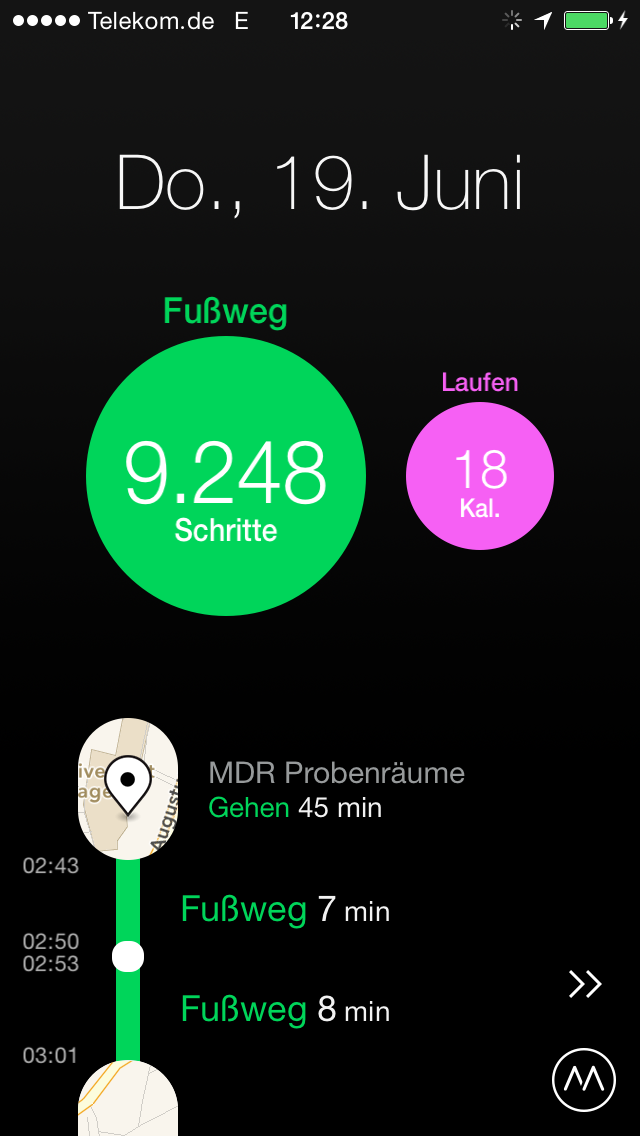
\includegraphics[scale=0.3]{images/moves-app-main-ui.PNG}
\caption{Moves Haupt-UI \cite{fig:Haupt-UI}}
\label{fig:Haupt-UI}
\end{figure}

\subsection{Design und Features}
%% ==============================
\label{ch:Apps:sec:Moves:subsec:DuF}

Moves hebt sich von den mittlerweile massenhaft existierenden Bezahl-Fitness-Apps und diversen tragbaren Geräten, wie zum Beispiel Fitbit One, das Nike Fuelband oder dem Withings Pulse, insofern sehr stark ab, dass die Daten hier in sehr viel benutzerfreundlicherer Art und Weise präsentiert werden, als bei den zuvor genannten.
\\
Die App glänzt durch eine gute Umsetzung und ihrer Einfachheit. 
Viele andere Fitness-Apps bombardieren den Nutzer regelrecht mit den bereitgestellten bzw. erfassten Daten, um diesen „ruhig“ zu stellen. 
Moves hingegen nimmt einen ganz anderen Ansatz wahr. 
Dem Nutzer werden die Daten, die durch die täglichen Aktivitäten erhalten wurden, als „Handlung“ bzw. Timeline des Tages anschaulich präsentiert.
\\
Der Einsatz von Sensoren, wie zum Beispiel dem Beschleunigungsmesser, gepaart mit GPS- und WiFi machen es so der Applikation möglich, zwischen den verschiedenen Aktivitäten des Nutzers, sowie dessen Stadtorte zu unterscheiden. 
Die gewonnenen Daten werden auf den hauseigenen Servern der Firma gespeichert, auf denen unter anderem auch ein Teil der Daten analysiert wird. 
Bei täglicher Nutzung von Moves fallen so etwa 30 MB an Daten an, die auf die Server geschoben werden. 
Das heißt natürlich nicht, dass die Anwendung nur online genutzt werden kann und dadurch das monatliche Übertragungs-Volumen schmälert. 
Eine Volumenschonende Nutzung - also offline - ist möglich, da die App die notwendigen Daten auch so sammelt, diese aber erst analysieren und auswerten kann, wenn wieder eine aktive Verbindung zum Internet, z.B. durch WiFi, besteht.   
\\
Die Benutzeroberfläche ansich ist eher spärlich gehalten. 
Es gibt lediglich die „Storyline“ bzw. die Timeline, die herunterscrollbar ist. 
Weiterhin existieren dreierlei Kreistypen, die oberhalb der Timeline angebracht sind und die jeweilige Aktivität, wie Wandern, Radfahren oder Laufen, darstellt. 
Diese zeigen dem Nutzer neben den getätigten „Schritten“ auch die Menge an verbrauchten Kalorien und die zurückgelegte Strecke in Kilometern an. 
Weiterhin bietet die die App Moves die Möglichkeiten Fortschritte herauszukristallisieren, da man aktuelle Aktivitäten mit denen vom Vortag oder der Vorwoche vergleichen kann.   
\\
\ref{fig:Timeline}

\begin{figure}[h]
\centering
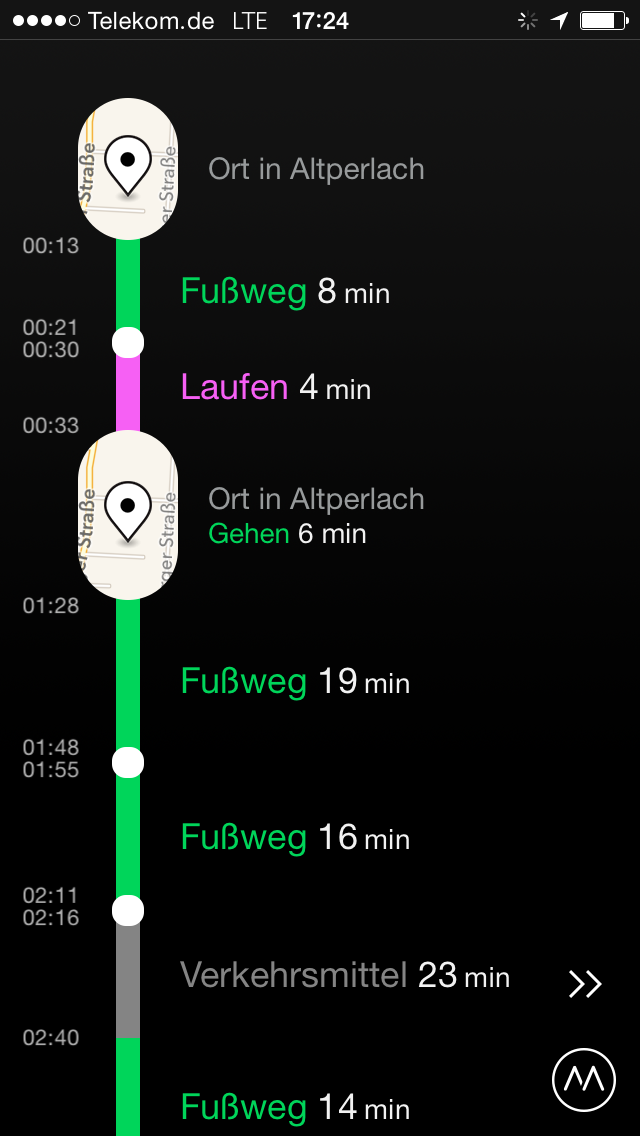
\includegraphics[scale=0.3]{images/moves_app_screenshot.png}
\caption{Moves Timeline \cite{fig:Timeline}}
\label{fig:Timeline}
\end{figure}

Die Einstellungen der Applikation sind ziemlich minimalistisch gehalten, da der Nutzer lediglich die Möglichkeiten hat, die Batterielebensdauer durch die Auswahl des stationären Einsatzes zu minimieren, die Messeinheiten zwischen „metrisch“ und „imperial“ ändern und einen täglich Aktivitätsbericht als Benachrichtigung erhalten kann. 
\\
Die Einbindung durch sogenannte „Third-Party-Apps“, also von Anwendungen anderer Hersteller, ist seit Anfang 2014 möglich und erweitert das Repertoire von Moves enorm. 
So ist die Einbindung von bis zu 13 anderen Apps, wie TicTrac oder Bounts derzeit möglich.  
\\
\ref{fig:Anwendungen}

\begin{figure}[h]
\centering
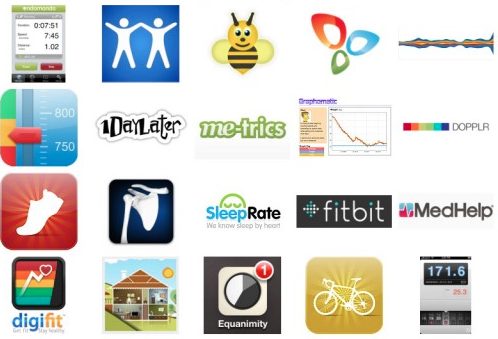
\includegraphics[scale=0.3]{images/qs-anwndungen-gadgets.png}
\caption{Verschiedene QS Anwendungen und Gadgets \cite{fig:Anwendungen}}
\label{fig:Anwendungen}
\end{figure}

\subsection{Die Performance}
%% ==============================
\label{ch:Apps:sec:Moves:subsec:PERF}

Das Großartige an der App Moves ist, dass der Nutzer kein extra Gerät - wie eine „Uhr“ am Handgelenk - benötigt, um die Datengenerierung zu ermöglichen, sondern lediglich das Smartphone bzw. Tablet des Nutzers alleine genügt. 
Auch wird durch das „Always-on“-Prinzip, also dass die Anwendung durchgehend im Hintergrund geöffnet ist, die ständige Datengenerierung gewährleistet, auch wenn der Nutzer einmal vergessen sollte, Moves zu öffnen.
\\
Da die Genauigkeit der Daten offensichtlich ein wichtiges Anliegen der Entwickler ist, zeigt sich im Vergleich mit der Tracking-App Withings Pulse, der einen Unterschied von ganzen 200 Schritten zeigte. 
Auch in Hinblick auf die angezeigte Distanz und Dauer war Moves so akkurat wie ein modernes TomTom GPS-Navigationsgerät.
\\
\ref{fig:GPS-Map}

\begin{figure}[h]
	\centering
	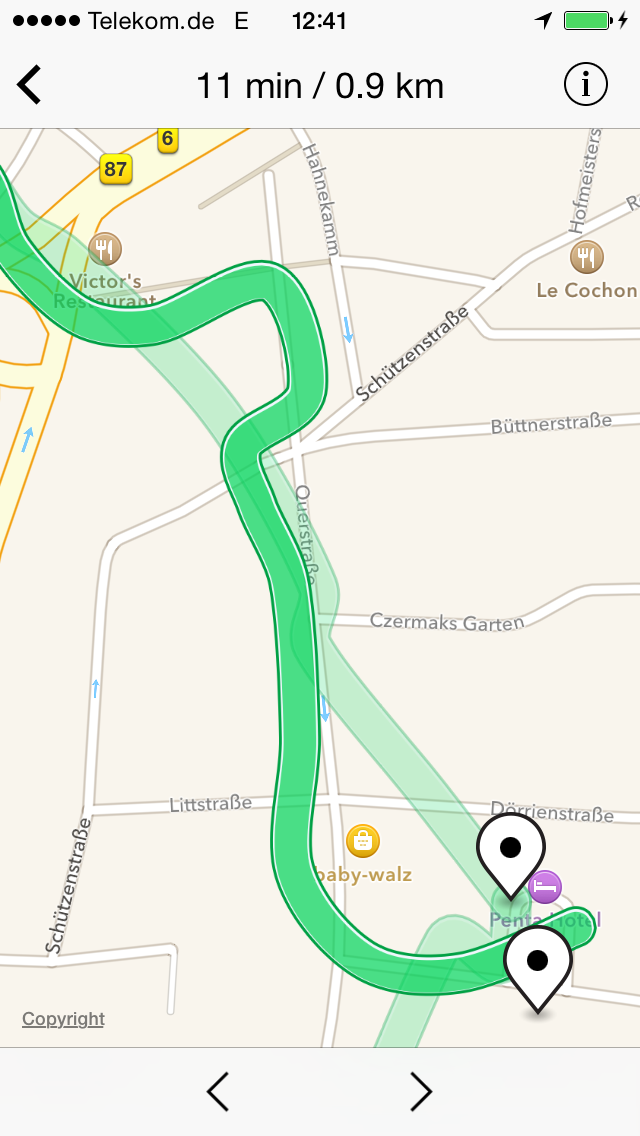
\includegraphics[scale=0.3]{images/moves-app-map.PNG}
	\caption{Moves GPS-Map \cite{fig:GPS-Map}}
	\label{fig:GPS-Map}
\end{figure}

Wie bei den meisten Apps, die sehr stark auf GPS setzen, um reibungslos funktionieren zu können, geht die Moves-Nutzung derweil stark auf die Akkulaufzeit des Smartphones/Tablets, was sich trotz verbesserter Technologie im Zusammenhang mit dem M7-Chip des iPhone 5S sehr bemerkbar macht. 
So raten die Entwickler den Nutzern, das Smartphone/Tablet immer über Nacht aufladen zu lassen bzw. den stationären Einsatz einzustellen.
\\
Der normalen täglichen Nutzung der App tut die etwas verkürzte Akkulaufzeit aber kein Abbruch. 
Man sollte lediglich darauf achten, andere Anwendungen stets zu schließen.

\subsection{Zusammenfassung}
%% ==============================
\label{ch:Apps:sec:Moves:subsec:VERDICT} 

Die Moves-App wird den Nutzer vielleicht nicht sofort fitter machen, das ist ja auch nicht die grundlegende Idee hinter der App. 
Es geht vielmehr darum, dem Nutzer ein „gesünderes“ Denken durch die Nutzung der Anwendung mit auf den Weg zu geben. 
So kann sich der Nutzer erstmal ein klareres Bild seiner Tagesaktivitäten und Bewegungen machen und so in die Lage versetzt werden, etwas an seinen Aktivitäten zu ändern bzw. zu verbessern.
\\
So eignet sich die App Moves trotz der kleinen Macken, wie Innennutzung oder Akkulaufzeit, sehr gut um mit einer gesünderen veränderten Aktivitätsplanung ins weitere Leben zu starten und schont zugleich den Geldbeutel, da der Nutzer auf die Anschaffung eines teuren Fitness-Tracking-Geräts verzichten kann.

%% ==============================
\section{Hueman}
%% ==============================
\label{ch:Apps:sec:Hueman}

\subsection{Was ist Hueman?}
%% ==============================
\label{ch:Apps:sec:Hueman:subsec:WIH}

Human ist eine weitere mobile QS-Anwendung, mit der sich das allgemeine tägliche Befinden tracken lässt. 
Durch die dadurch gewonnen Daten soll der Nutzer etwaige positive oder negative Veränderungen durch bestimmte Aktivitäten erkennen und besser einordnen.
Seit Anfang 2014 ist die Applikation in Apples' AppsStore erhältlich, um die Gemütszustände zu erfassen.


\subsection{Design und Features}
%% ==============================
\label{ch:Apps:sec:Hueman:subsec:DuFe}

Auch die Entwickler dieser Anwendung schreiben das Wort "simplicity" groß. 
Denn durch einfaches Wischen des Nutzers über den Bildschirm des Smartphones legt dieser seinen aktuellen Gefühlszustand fest.
\ref{fig:HUI}

\begin{figure}[h]
	\centering
	
\includegraphics[scale=0.3]{images/hueman-app-main-ui.PNG}
	\caption{Hueman UI \cite{fig:HUI}}
	\label{fig:HUI}
\end{figure}

Optisch aufgewertet werden die einzelnen Zustande durch eine Art Farbpalette, bei der die „waren“ Farben für eine gute bis sehr gute und die „kalten“ Farben für die schlechte bis miserable Stimmung stehen.
Die Applikation vergleicht die einzelnen gewonnenen Daten miteinander und gibt diese dem Nutzer als fortlaufendes Diagramm aus, sodass er die Veränderungen der Stimmungen schnell erkennen kann.
\ref{fig:Vergleich}

\begin{figure}[h]
\centering
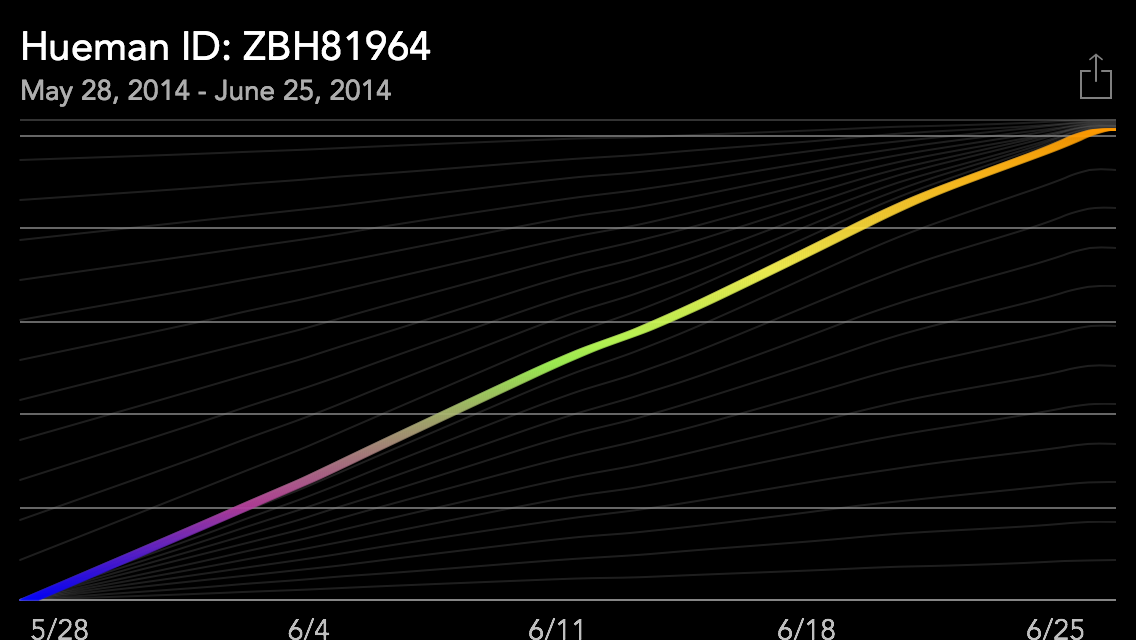
\includegraphics[scale=0.3]{images/hueman-matched-data.PNG}
\caption{Hueman Vergleich \cite{fig:Vergleich}}
\label{fig:Vergleich}
\end{figure}


\subsection{Zusammenfassung}
%% ==============================
\label{ch:Apps:sec:Hueman:subsec:Verdict}

Da sich die App Hueman leicht und vor allem schnell bedienen lässt, ist sie der optimale Begleiter für Nutzer, die gerne mehr über die Wechselwirkungen ihrer Stimmung Bescheid wissen wollen.
Sie erlaubt es durch einfache grafische Aufwertungen, dem Nutzer auch visuell seine Stimmungen näher zubringen.  


%% ==============================
\section{Sleep Cycle}
%% ==============================
\label{ch:Apps:sec:SleepCycle}

Sleep Cycle ist ein Schlafphasenwecker, welcher das Schlafmuster des Benutzers analysiert und in der leichtesten Phase des Schlafes aufweckt. \cite{web:SleepCycle}
Dafür zeichnet die Software die Bewegungsaktivitäten während des Schlafes auf und wertet diese aus.
Darüber hinaus biete die Applikation zusätzliche Möglichkeiten um die Schlafgewohnheiten zu Kategorisieren sowie die Auswirkungen in unterschiedliche Charts zu begutachten. 
Die Idee von intelligenten Schlafphasenweckern besteht darin, die Schlafgewohnheit aufzuzeichnen und mit Notizen zu versehen. Dadurch erlangt man die Erkenntnis über die Schlafqualität in Zusammenhang mit deren Ursachen, um im Anschluss die eignen Gewohnheiten zu verändern, damit die Qualität des Schlafes zu verbessern und sich erholter zu fühlen.

\subsection{Hintergrundwissen}
\label{ch:Apps:sec:Sleepcycle:subsec:H}

Der Schlaf ist ein wichtiges aktiver Teiles des täglichen Lebens und dient der Erholung von Körper und Geist.
Bei zu wenig Schlaf leidet der Körper unter Schlafmangel und kann zu Depressionen, Bluthochdruck oder weiteren Krankheiten führen. \cite{Chen:SleepMonitoring}

Das bereits ca. 15\% der Bevölkerung in Deutschland an immer wiederkehrenden Schlafstörungen leiden und dem Steigenden Interesse an \textbf{Quantified Self}, sind Gründe für immer mehr der sogenannten "Sleep Tracker" auf dem Markt. 
Mit diesen, als reiner Software auf dem Smartphone (Bsp. \textbf{Sleep Cycle \ref{ch:Apps:sec:SleepCycle}}) oder mit zusätzlicher Hardware (Bsp. JawboneUp), lässt sich der Schlaf des Benutzers analysieren und eventuelle Schwachstellen aufzeigen.

Praktisch bewegt sich der Mensch in den verschieden Phasen des Schlafes unterschiedlich stark.
Diese einzelnen Bewegungen zeichnet die Software „Sleep Cycle“ mit Hilfe des eingebauten „Accelerometer“ (dt. Beschleunigungssensor) des Aufzeichnungsgerätes (Smartphone) auf.
Der Schlaf wird generell in folgende 5 Stadien untergliedert:

\begin{itemize}
	\item Einschlafphase (1 Phase)
	\item Leichter Schlaf (2 Phase)
	\item Mittlerer Schlaf (3 Phase)
	\item Tiefer Schlaf (4 Phase)
	\item REM Schlaf (5 Phase)
\end{itemize}

Von Phase eins bis vier nehmen die Bewegungen der Muskel ab, bis diese während des REM Schlafes vollkommen versiegen.
Diese Zyklus dauert circa 90 Minuten und wird während des Schlafes mehrmals durchlaufen.
Dadurch lassen sich die einzelnen Phasen des Schlafes anhand der Bewegung bestimmen. \textbf{BELEGEN}
Innerhalb der ersten beiden Phasen befindet sich der Körper in Momenten in denen er fast Wach ist. Zu diesem Zeitpunkt ist der Benutzer am leichtesten zu Wecken und fühlt sich ausgeschlafener und erholter.
Mit Hilfe der ermittelten Phase und dem gewählten Weckzeitraum, ertönt der Wecker sobald sich der Benutzer in der Leichtesten Phase des Schlafes befindet. Siehe Abbildung \ref{fig:Hypnogramm}


\begin{figure}[h]
\centering
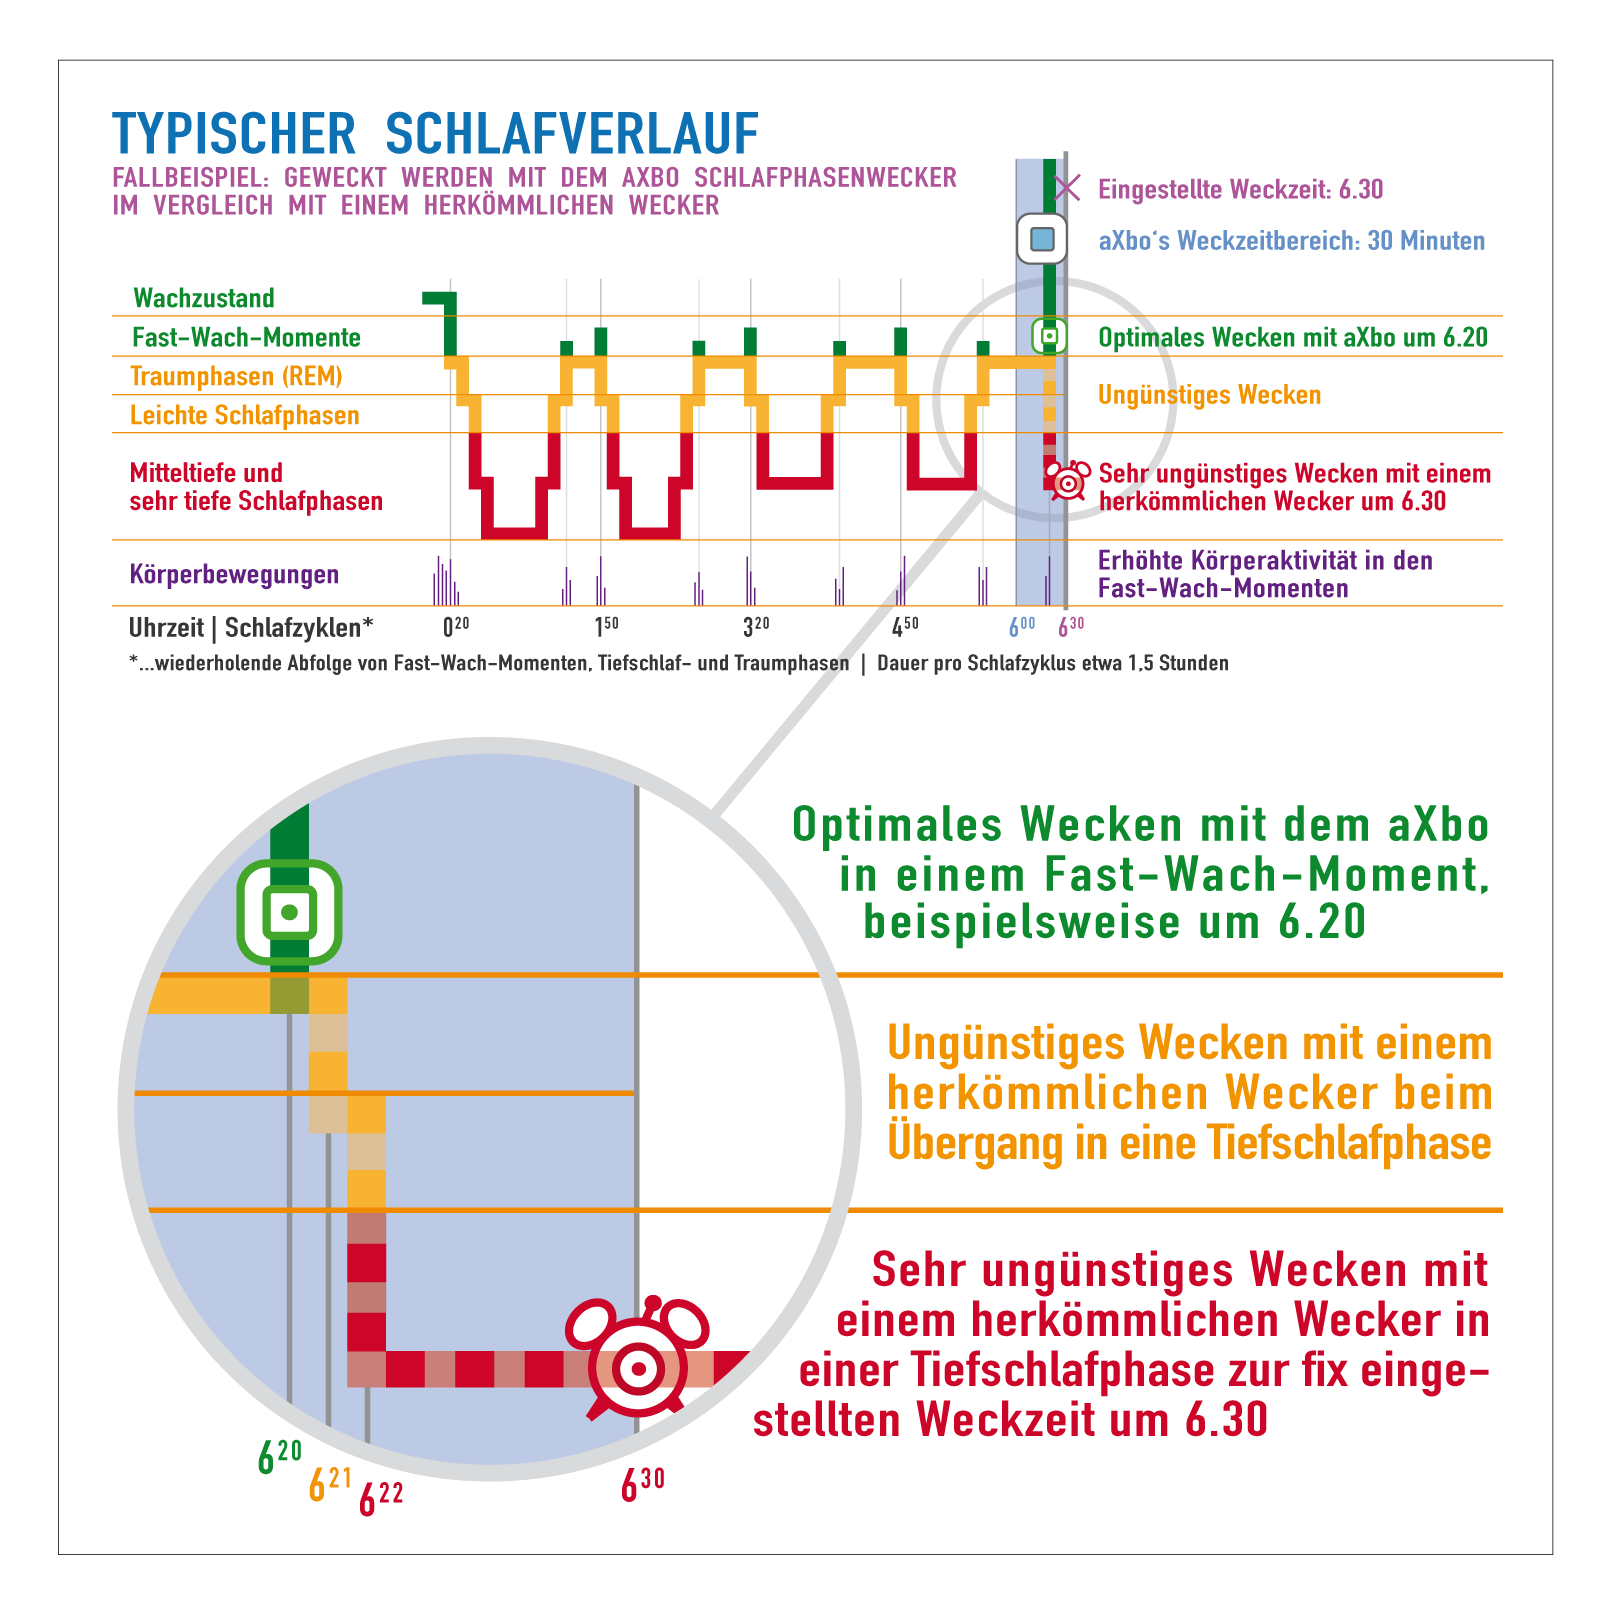
\includegraphics[width=0.9\textwidth]{images/aXbo_Schlafverlauf_Hypnogramm_DE.png}
\caption{Schlafverlauf Hypnogramm \cite{fig:Hypnogramm}}
\label{fig:Hypnogramm}
\end{figure}


\subsection{Funktionsweise und Anwendung}
\label{ch:Apps:sec:Sleepcycle:subsec:FuA}

Um das Ziel eines Schlafphasenweckers zu erreichen, bietet \textbf{Sleep Cycle} mehrere Funktionen und Anwendungsszenarien an.
Die Hauptfunktion ist die Aktivierung des Alarms. \ref{fig:SCAlarm}
Hier wird die späteste Weckzeit gewählt und der Zeitraums des gesamten Weckvorgangs angezeigt.
Die Standardeinstellung für den Weckzeitraum beträgt 30 Minuten.
Nach dem setzen des Weckers erscheint die Sleep Note Today Ansicht \ref{fig:SCSleepNoteToday}, welche der Kategorisierung des Tages vor dem Schlaf dient. Dadurch lassen sich Rückschlüsse auf die täglichen Gewohnheiten schließen und die darauffolgende Schlafqualität beurteilen.

\begin{figure}[]
  \centering
  \begin{minipage}[b]{0.47\textwidth}
    \centering
    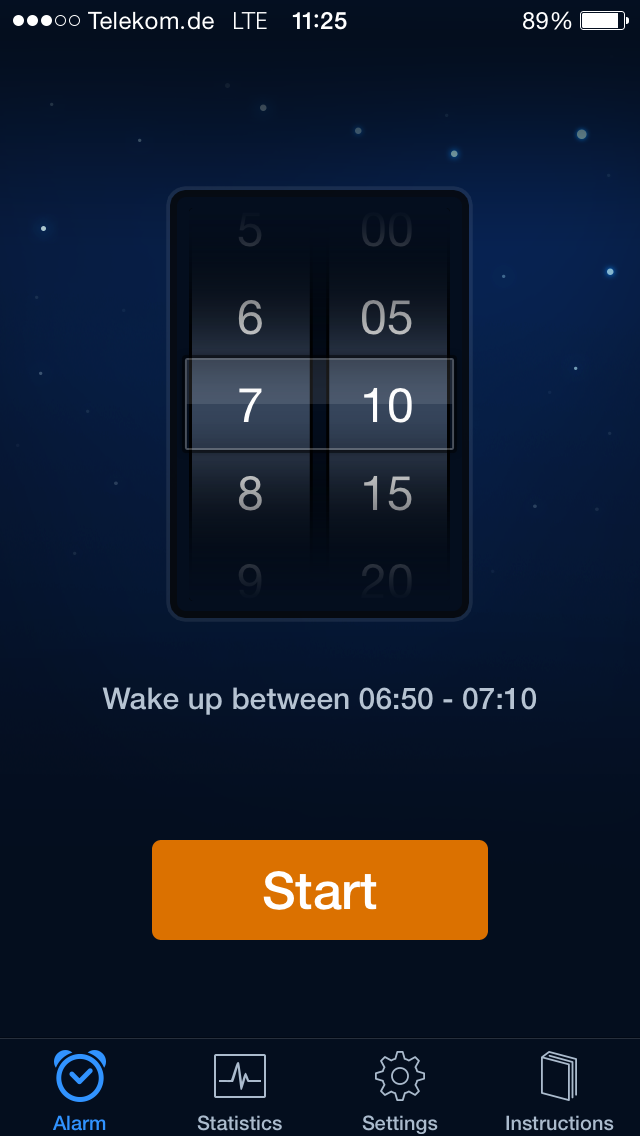
\includegraphics[scale=0.3]{images/SleepCycle/Alarm} 
    \caption{Sleep Cycle Alarm}
    \label{fig:SCAlarm}
  \end{minipage}
  \begin{minipage}[b]{0.47\textwidth}
    \centering
    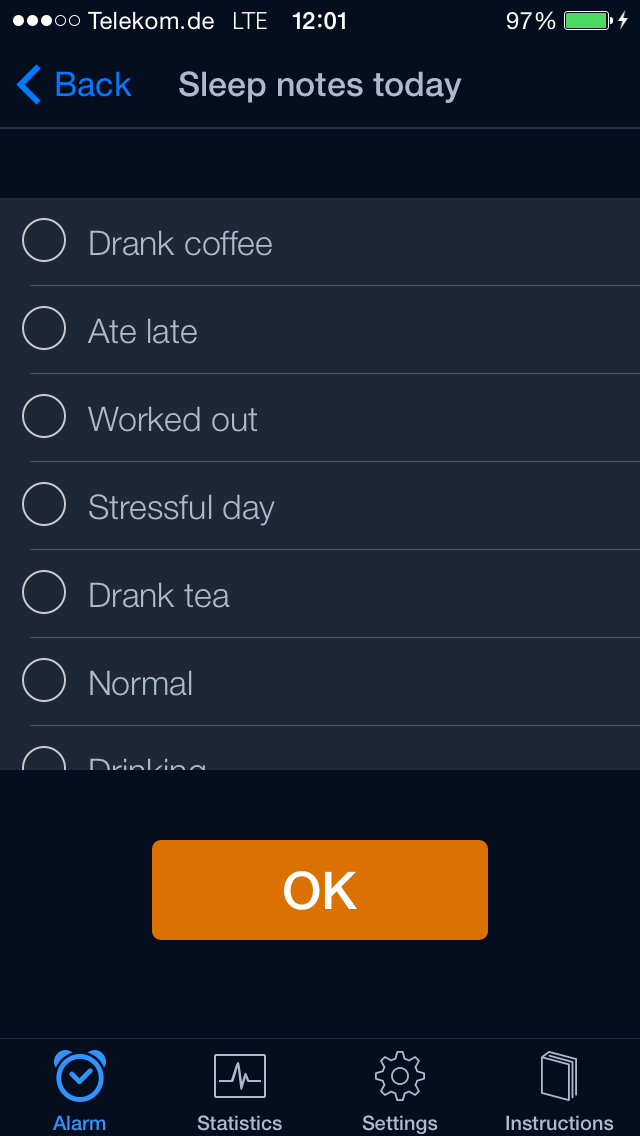
\includegraphics[scale=0.3]{images/SleepCycle/SleepNotesToday}  
    \caption{Sleep Cycle Sleep Note}
    \label{fig:SCSleepNoteToday}
  \end{minipage}
\end{figure}

Zusätzlich bietet \textbf{Sleep Cylce} weitere Einstellungs, Tracking und Analyse Funktionen, die dem Erfolgreichen Auswerten dienen.
In den Einstellung lassen sich unterschiedliche Möglichkeiten des Weckens wählen, sowie zusätzliche Sinnvolle Features aktivieren, mit den die Analyse vereinfacht werden kann.
Zum einen lässt sich die Stimmung des Benutzer aufwehmen, wie leicht er aufgewacht ist.
Zum anderen 


Diese zeigen dem Nutzer Informationen über deren Schlaf sowie Mögliche Ursachen für Störung.
Dafür analysiert die Software die Bewegungen während des Schlafes und erfasst Informationen über den Vergangen Tag des Benutzers.
Alle erfassten Daten werden in unterschiedlichen Grafiken dargestellt.

 

\begin{figure}[]
  \centering
  \begin{minipage}[b]{0.47\textwidth}
    \centering
    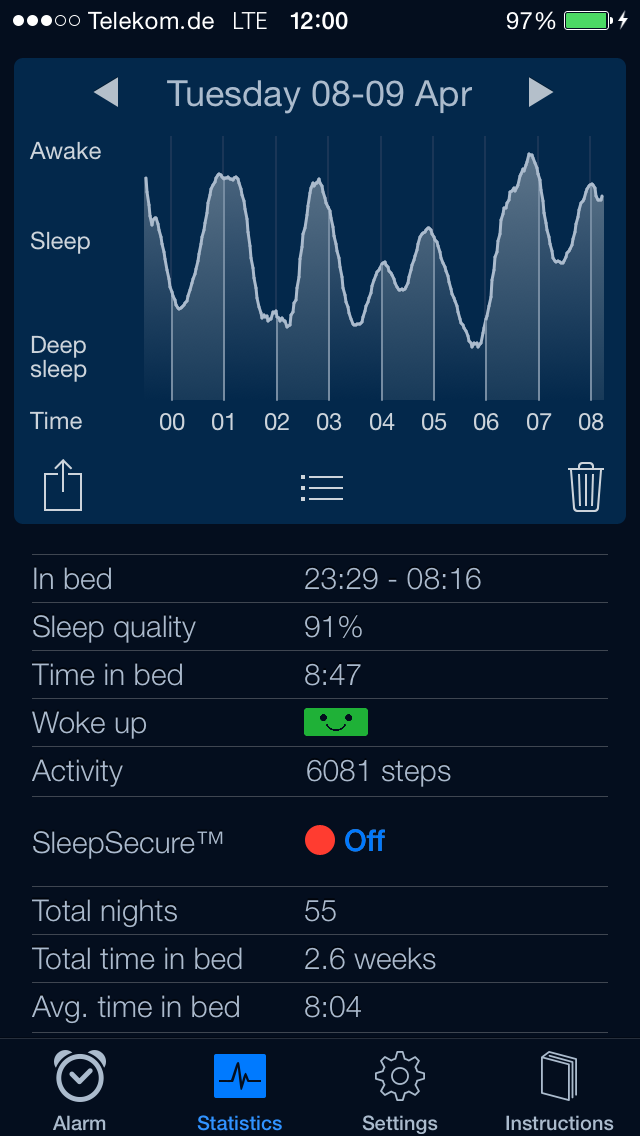
\includegraphics[scale=0.3]{images/SleepCycle/Detail} 
    \caption{Sleep Cycle Detail}
    \label{fig:SCDetail}
  \end{minipage}
  \begin{minipage}[b]{0.47\textwidth}
    \centering
    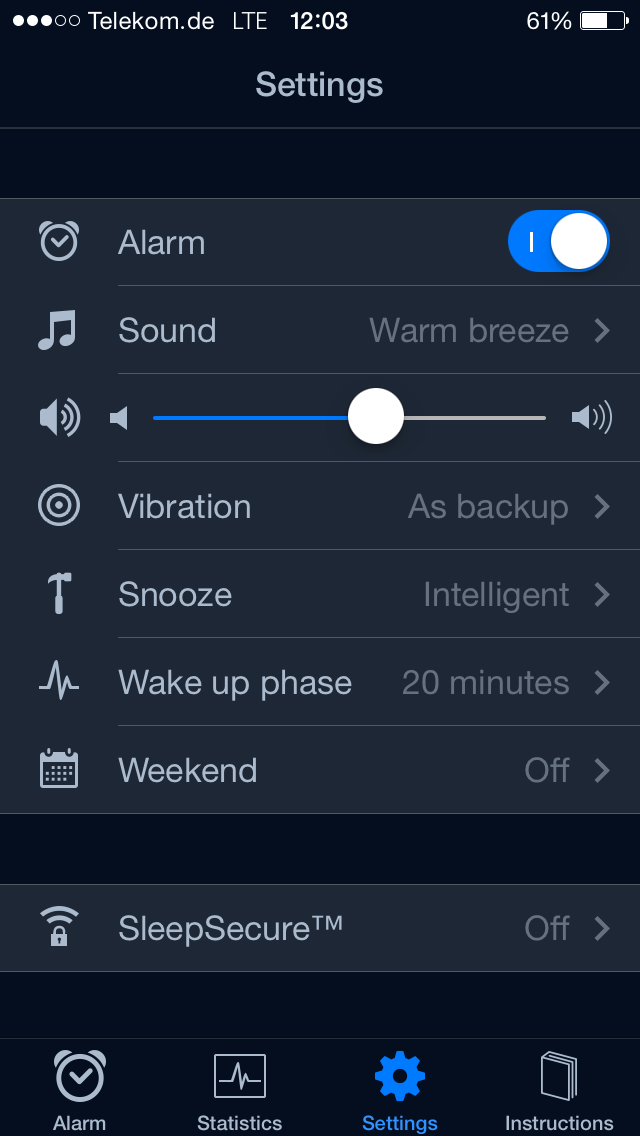
\includegraphics[scale=0.3]{images/SleepCycle/Settings1}  
    \caption{Sleep Cycle Settings}
    \label{fig:SCSettings}
  \end{minipage}
\end{figure}

\begin{figure}[]
	\centering
    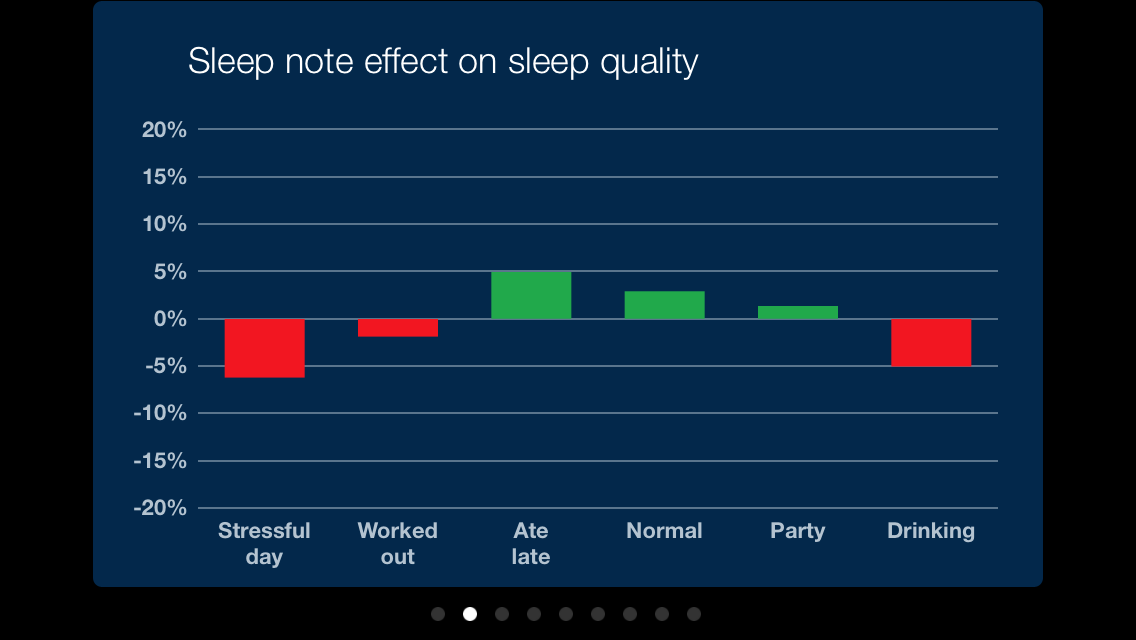
\includegraphics[scale=0.3]{images/SleepCycle/SleepNoteEffectOnSleepQuality} 
    \caption{Sleep Cycle Sleep note effect}
    \label{fig:SCDetail}
\end{figure}

\begin{figure}[]
    \centering
    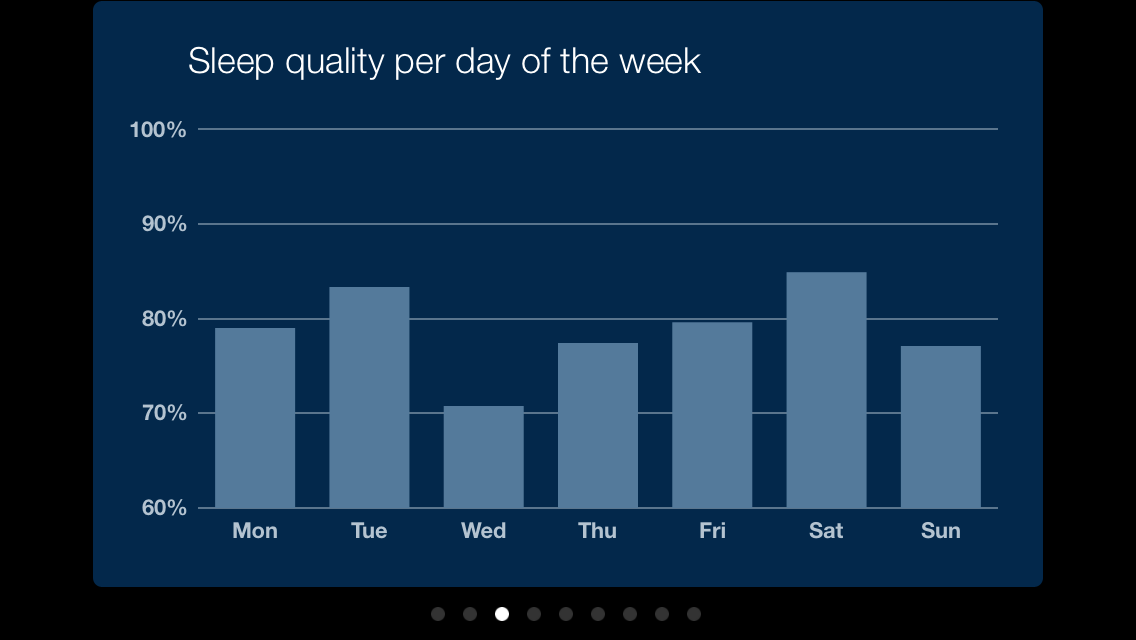
\includegraphics[scale=0.3]{images/SleepCycle/SleepQualityPerDayOfWeek}  
    \caption{Sleep Cycle Sleep quality per day of week}
    \label{fig:SCSettings}
\end{figure}


%%% Local Variables: 
%%% mode: latex
%%% TeX-master: "thesis"
%%% End: 

%% relativ.tex
%% $Id: analyse.tex 61 2012-05-03 13:58:03Z bless $

%% ==============================
\chapter{Relativierung}
%% ==============================
\label{ch:Relativierung}

Diese Kapitel beschäftigt sich mit möglichen Fehlerquellen die während der Datenerhebung und Auswertung auftreten können. 
Dabei wird Unterschieden in technische, sowie statistische Schwierigkeiten die während der Aufzeichnungsphase im Projekt auftreten können.

%% ==============================
\section{Systematische und zufällige Fehler}
%% ==============================
\label{ch:Relativierung:sec:SystematischeUndZufälligeFehler}

Vor und während der Erhebung der Daten können unterschiedliche technische Probleme auftreten.
Unterschieden werden diese in systematische und zufällige Fehler.

Diese werden im Folgenden näher erläutert.

\subsection{Kalibirierung}
%% ==============================
\label{ch:Relativierung:sec:SystematischeUndZufälligeFehler:subsec:Kalibrierung}
%% ==============================

Zu Beginn der Aufzeichnungsphase initialisieren die Apps Moves \ref{ch:Apps:sec:Moves} und Sleep Cycle \ref{ch:Apps:sec:SleepCycle} die Kalibrierung.
Diese sollte von dem jeweiligen Nutzer des Quantified Self Tools selbst durchgeführt werden.
Eine fehlenede oder  falsche Kalibrierung der Software bzw. Hardware ist ein systematischer Fehler, er führt zu einer Verzerrung der erhobenen Daten und im weiteren Schritt zu einer unzutreffenden Interpretation des Ergebnis.
Diese fehlerhaften Resultate können die Beantwortung der Leitfrage somit negativ beeinflussen. 


\subsection{Ausfallsicherheit}
%% ==============================
\label{ch:Relativierung:sec:SystematischeUndZufälligeFehler:subsec:Ausfallsicherheit}
%% ==============================

Im Verlauf der Aufzeichnung kann es zu weiteren Fehlern kommen.
Durch die Benutzung von Sensoren und Techniken für Ortung und Bewegung des Aufzeichnungsgerätes, steigt die Belastung der benutzten Akkumulatoren.
Der gesteigerte Energieverbrauch kann während eines durchschnittlichen Alltag zu einer vorzeitigen Notwendigkeit des Ladevorgangs führen.
Fällt das Gerät wegen eines Hardware-, Softwarefehlers oder mangelnder Stromversorgung aus, so fehlen Daten die wiederum das Endergebnis verfälschen.

\subsection{Genauigkeit}
%% ==============================
\label{ch:Relativierung:sec:SystematischeUndZufälligeFehler:subsec:Genauigkeit}
%% ==============================

Die Genauigkeit der gewonnenen Daten hängt von vielen Faktoren ab. 
GPS-unterstützte Tracking-Applikationen, wie die für das Projekt ausgewählten, sind besonders  anfällig, ungenaue Daten zu generieren. 
So beträgt bei guten Empfangsbedingungen die erzielbare Genauigkeit ohne Korrektur etwa 5 bis 20m. 
Da aber die meisten gängigen GPS-Empfänger auch WAAS/EGNOS-Korrektursignale empfangen können, verbessert sich die tatsächlich erzielbare Genauigkeit auf 1 bis 3m. \\
Da optimale Empfangsbedingungen jedoch nicht häufig erreicht  werden ist die Genauigkeit dieser Apps sehr umstritten.
Dies liegt unter anderem daran, dass sich die GPS-Funkwellen sich aufgrund der sehr hohen Frequenz quasi-optisch ausbreiten und der GPS-Empfänger deshalb immer zu möglichst vielen Satelliten Kontakt haben sollte. 
Daraus resultieren auch die meisten Fehler in der Positionsberechnung, die durch zu starke Dämpfung, Reflexion einzelner oder aller GPS-Signale und durch den Empfang von zu wenig Satelliten verursacht wird. \\
So ist zum Beispiel in Tälern oder in Häuserschluchten der Kontakt zum Himmel sehr eingeschränkt. 
Dadurch können weniger Satelliten empfangen werden und es treten sogenannte Reflexionen auf. 
Eine Dämpfung hingegen tritt zum Beispiel im Wald unter dichtem Blätterdach auf, oder auch wenn der GPS-Empfänger an einer ungünstigen Stelle im Fahrzeug positioniert wurde. \\
Im Gegensatz zu aktuell gängigen GPS-Empfängern, die sowohl den erfolgreichen Empfang des WAAS/EGNOS-Korrektursignals, als auch einen Schätzwert für die Genauigkeit der Positionsberechnung anzeigen, ist dies in den mobilen Applikationen nicht gegeben. 
Bei schlechten Empfangsbedingungen können sich diese Genauigkeitsangaben sehr von den wirklichen Daten unterscheiden.  
So kann sich die tatsächlich gelaufene Strecke von der in Moves angezeigten maßgeblich unterscheiden, da die Angabe dort eine Schnittmenge aus der Schrittanzahl und der GPS-Daten darstellt.\ref{fig:GPS-Map}


Erklärung Abkürzungen
WAAS: 
Wide Area Augmentation System ist in ein in Nord-Amerika genutztes bodengestütztes System, um GPS-Positionsabweichungen zu korrigieren
EGNOS: 
European Geostationary Navigation Overlay Service ist in ein in Europa genutztes bodengestütztes System, um GPS-Positionsabweichungen zu korrigieren

%% Lösung: Weitere Geräte, Redundanz, dedizierte Geräte

%% ==============================
\section{Statistische Schwierigkeiten}
%% ==============================
\label{ch:Relativierung:sec:StatistischeSchwierigkeiten}

Neben den technischen, systematischen und zufälligen Fehlern, können auch statistische Schwierigkeiten das Experiment beeinflussen.
Beispielsweise handelt es sich bei einem empirischen Selbstversuch von drei Personen nicht um eine repräsentative Probe.
Auch ist der Zeitraum der Datenerhebung mit etwa einem Monat zu kurz um eine Veränderung des Nutzers festzustellen.
Diese Probleme ließe sich jedoch durch eine größere Anzahl an Testpersonen und einen längeren Zeitraum einfach lösen.
Außerdem könnte man durch eine Kontrollgruppe das Ergebnis mit der Quantified Self Gruppe besser vergleichen. 


%% probleme: partner im bett, zeitraum, mehr testpersonen, leider keine repräsentative 
%% lösung: vergleichsgruppe, mehr zeit/längerer zeitraum,

%% Lösung: Testgruppen



%%% Local Variables: 
%%% mode: latex
%%% TeX-master: "thesis"
%%% End: 



 	  %Fehleranalyse
%%% eval.tex
%% $Id: eval.tex 61 2012-05-03 13:58:03Z bless $

\chapter{Evaluierung}
\label{ch:Evaluierung}
%% ==============================
Hier kommt der Nachweis, dass das in Kapitel~\ref{ch:Entwurf}
entworfene Konzept auch funktioniert. Leistungsmessungen einer
Implementierung werden auch immer gerne gesehen.

Bla fasel\ldots

%% ==============================
\section{Abschnitt 1}
%% ==============================
\label{ch:Evaluierung:sec:Abschnitt1}

Bla fasel\ldots

%% ==============================
\section{Abschnitt 2}
%% ==============================
\label{ch:Evaluierung:sec:Abschnitt2}

Bla fasel\ldots

%% ==============================
\section{Zusammenfassung}
%% ==============================
\label{ch:Evaluierung:sec:zusammenfassung}

Am Ende sollten ggf. die wichtigsten Ergebnisse nochmal in \emph{einem}
kurzen Absatz zusammengefasst werden.

%%% Local Variables: 
%%% mode: latex
%%% TeX-master: "thesis"
%%% End: 
        % Evaluierung
%% analyse.tex
%% $Id: analyse.tex 61 2012-05-03 13:58:03Z bless $

\chapter{Analyse und Evaluierung}
\label{ch:AnalyseUndEvaluierung}
%% ==============================

Die Beantwortung der Leitfrage des Projekts, ob durch Quantified Self das Wohlbefinden verbessert werden kann, hängt maßgeblich von einer genauen Analyse der Daten ab. 
Die zuvor in der Datengenerierungsphase erhobenen Daten müssen unter Berücksichtigung etwaiger Fremdeinflüsse bzw. Verfälschungen analysiert und ausgewertet werden.
Um dies zu gewährleisten sind wichtige Anforderungen an die Analyse gestellt, auf die im Folgenden näher eingegangen wird.

Exemplarische wurden nun nachdem alle Daten analysiert und ausgewertet wurden eine Testperson ausgewählt, anhand der die Leitfrage „Lässt sich das Wohlbefinden durch Quantified Self verbessern?“ beantwortet werden soll.

Aufgrund einer in der Gesamtheit Neuerhebung von Daten, liegt bei deren Auswertung der Fokus auf der deskriptive Datenanalyse.

\begin{quote}
Deskriptive Datenanalyse: Liegt eine Totalerhebung oder generell ein Datensatz vor, so ist es die Aufgabe der Datenanalyse, die in den Einzeldaten enthaltene Information zu verdichten und diese so darzustellen, dass Wesentliches deutlich wird. Dazu werden Tabellen, graphische Darstellungen und charakteristische Maßzahlen verwendet.  Die Datenanalyse hat ausschließlich beschreibenden Charakter (deskriptive Statistik). 
\end{quote}
\cite{http://wirtschaftslexikon.gabler.de/Definition/datenanalyse.html?referenceKeywordName=statistische+Datenanalyse}


Laut Schäfer\cite{Schafer2010} ist im Anschluss der deskriptiven Datenanalye mit der explorativen Statistik fortzufahren.
Dabei wird versucht Muster zu erkennen, welche mit Hilfe von Grafiken und Daten beschrieben werden.
Abschließend wird mit der Inferenzstatistik die Auswertung vollendet.
In diesem letzten Schritt wird versucht mit Hilfe von Stichprobendaten auf die allgemeine These zu schließen.

Dazu wurden verschiedene Korrelationskoeffizienten berechnet und Graphen erstellt.


%% ==============================
\section{Zusammenhang Schlafqualität und Schritte pro Tag}
%% ==============================
\label{ch:AnalyseUndEvaluierung:sec:ZusammenhangSchlafqualitätProSchrittenAmTag}

\begin{figure}[H]
\centering
        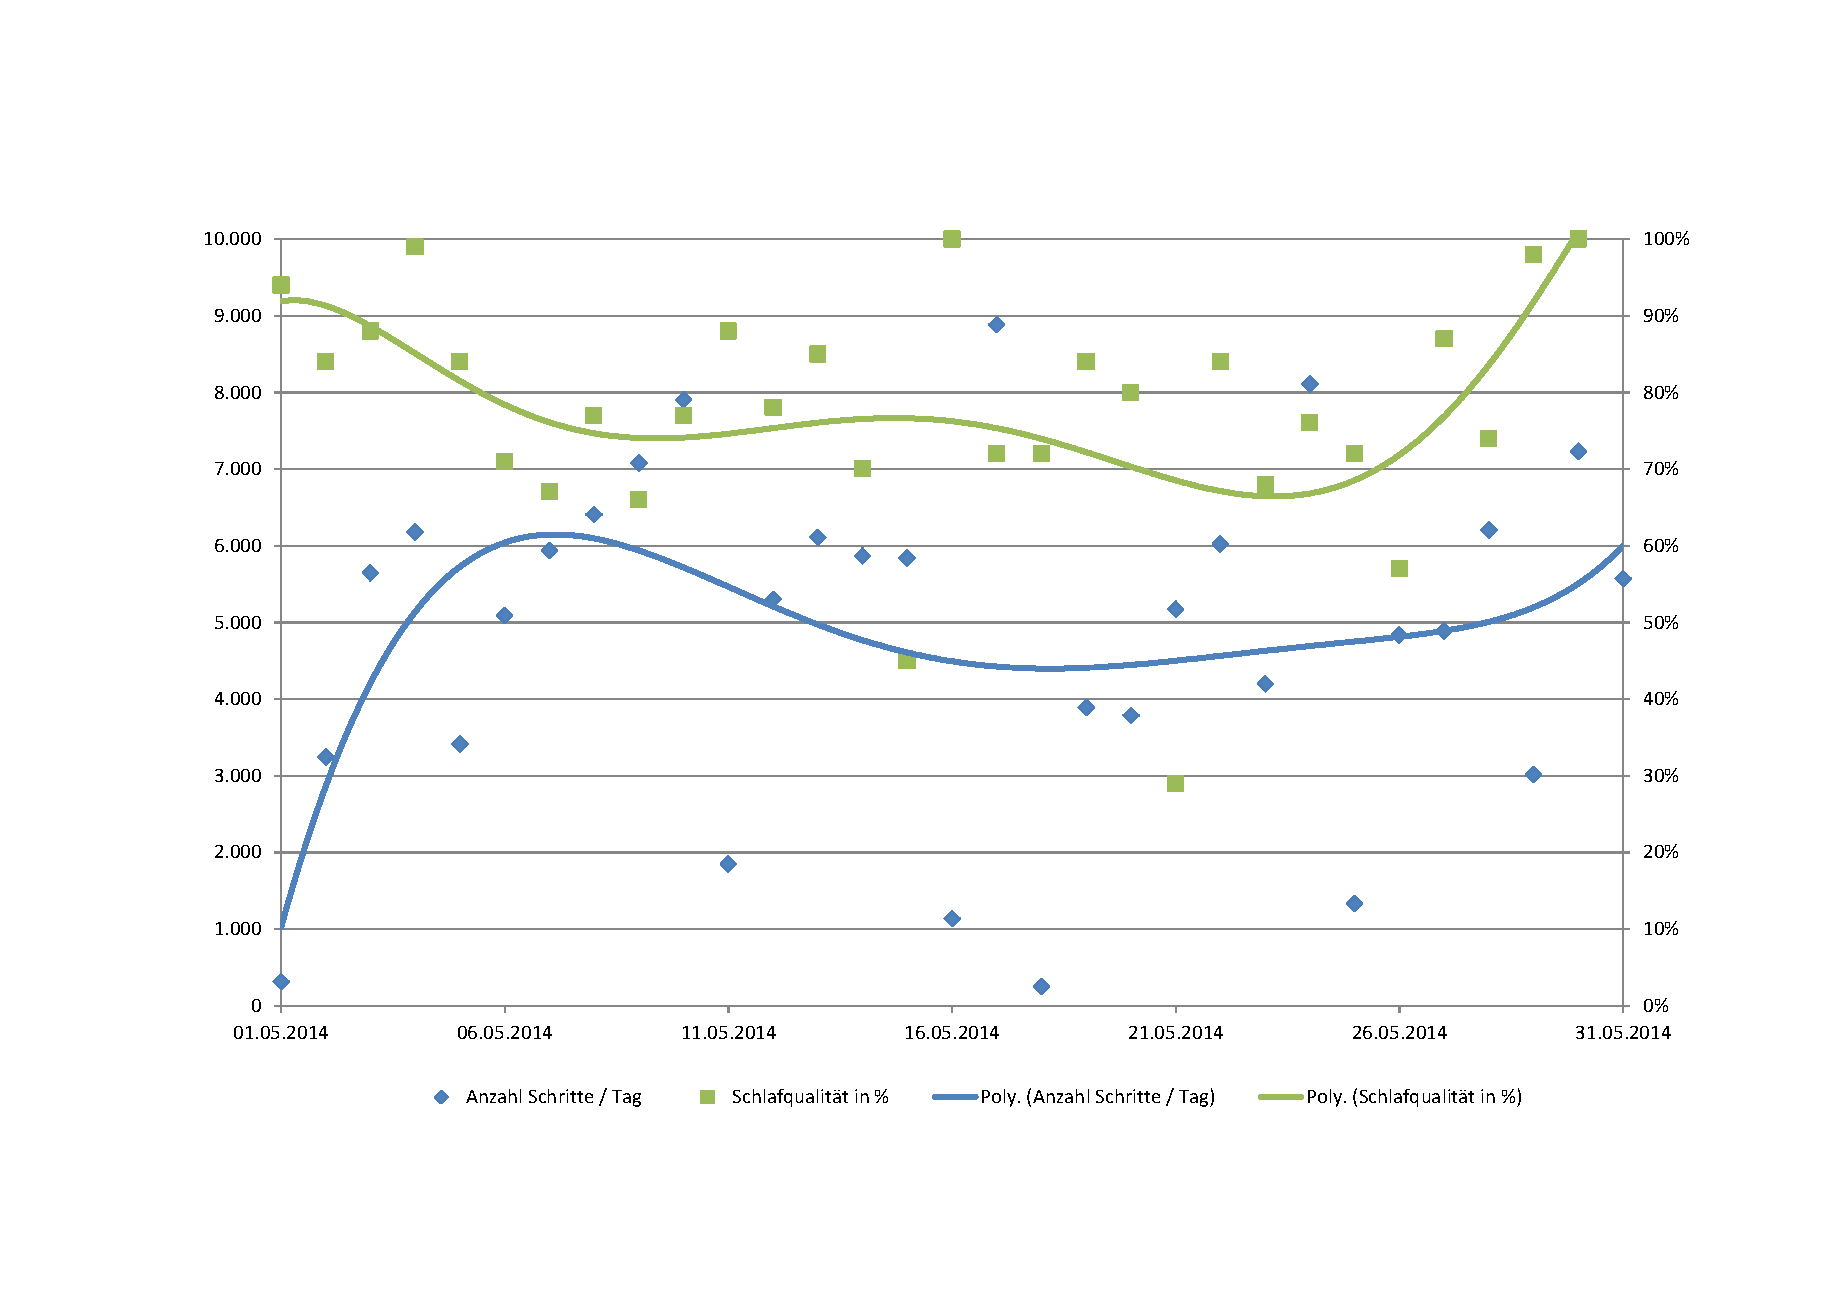
\includegraphics[angle=270,width=0.9\textwidth]{images/Analyse/Sleep-Steps} 
        \caption[Daten der Schritte pro Tag und der Schlafqualität]{Daten der Schritte pro Tag und der Schlafqualität}
        \label{fig:ZusammenhangSchlafqualitätProSchrittenAmTag}
\end{figure}

Das Diagramm \ref{fig:ZusammenhangSchlafqualitätProSchrittenAmTag} zeigt die Anzahl der aufgenommen Schritte pro Tag und zusätzlich die Schlafqualität in Prozent des jeweiligen Tages.
Die Werte der Grafik beziehen sich auf den kompletten Aufzeichnugszeitraums. 
Dabei handelt es sich bei den grünen Punkten um die einzelnen Datenpunkte der Schlafqualität, welche in Prozent auf der rechten Abzissenachse angegeben ist.
Auf der linken Abzissenachse wiederum wird die gesamte Anzahl der Schritte gezeigt, wie es auch der Legende zu entnehmen ist.
Zur besser Trend Ersichtlichkeit sind beide Datenreihen zusätzlich in einem Polynom sechsten Grades angenähert.
Diese Werte sind über den Erhebungszeitraum dargestellt.

Die Daten stammen aus dem Monat Mai des Jahres 2014.
In der Abbildung stamme die Werte Schritte pro Tag aus der im Projekt verwendeten Applikation Moves[\ref{ch:Apps:sec:Moves}]. 
Sleep Cycle[\ref{ch:Apps:sec:SleepCycle}] liefert dabei die Daten zur Schlafqualität.
Die Werte wurden im Zuge des Projektes von den Autoren erhoben.



%% ==============================
\section{Zusammenhang von Stimmung, Schlafqualität und Energieverbrauch}
%% ==============================
\label{ch:AnalyseUndEvaluierung:sec:KorrelationVonSchlafqualitätUndSchrittenAmTag}

\begin{figure}[H]
\centering
        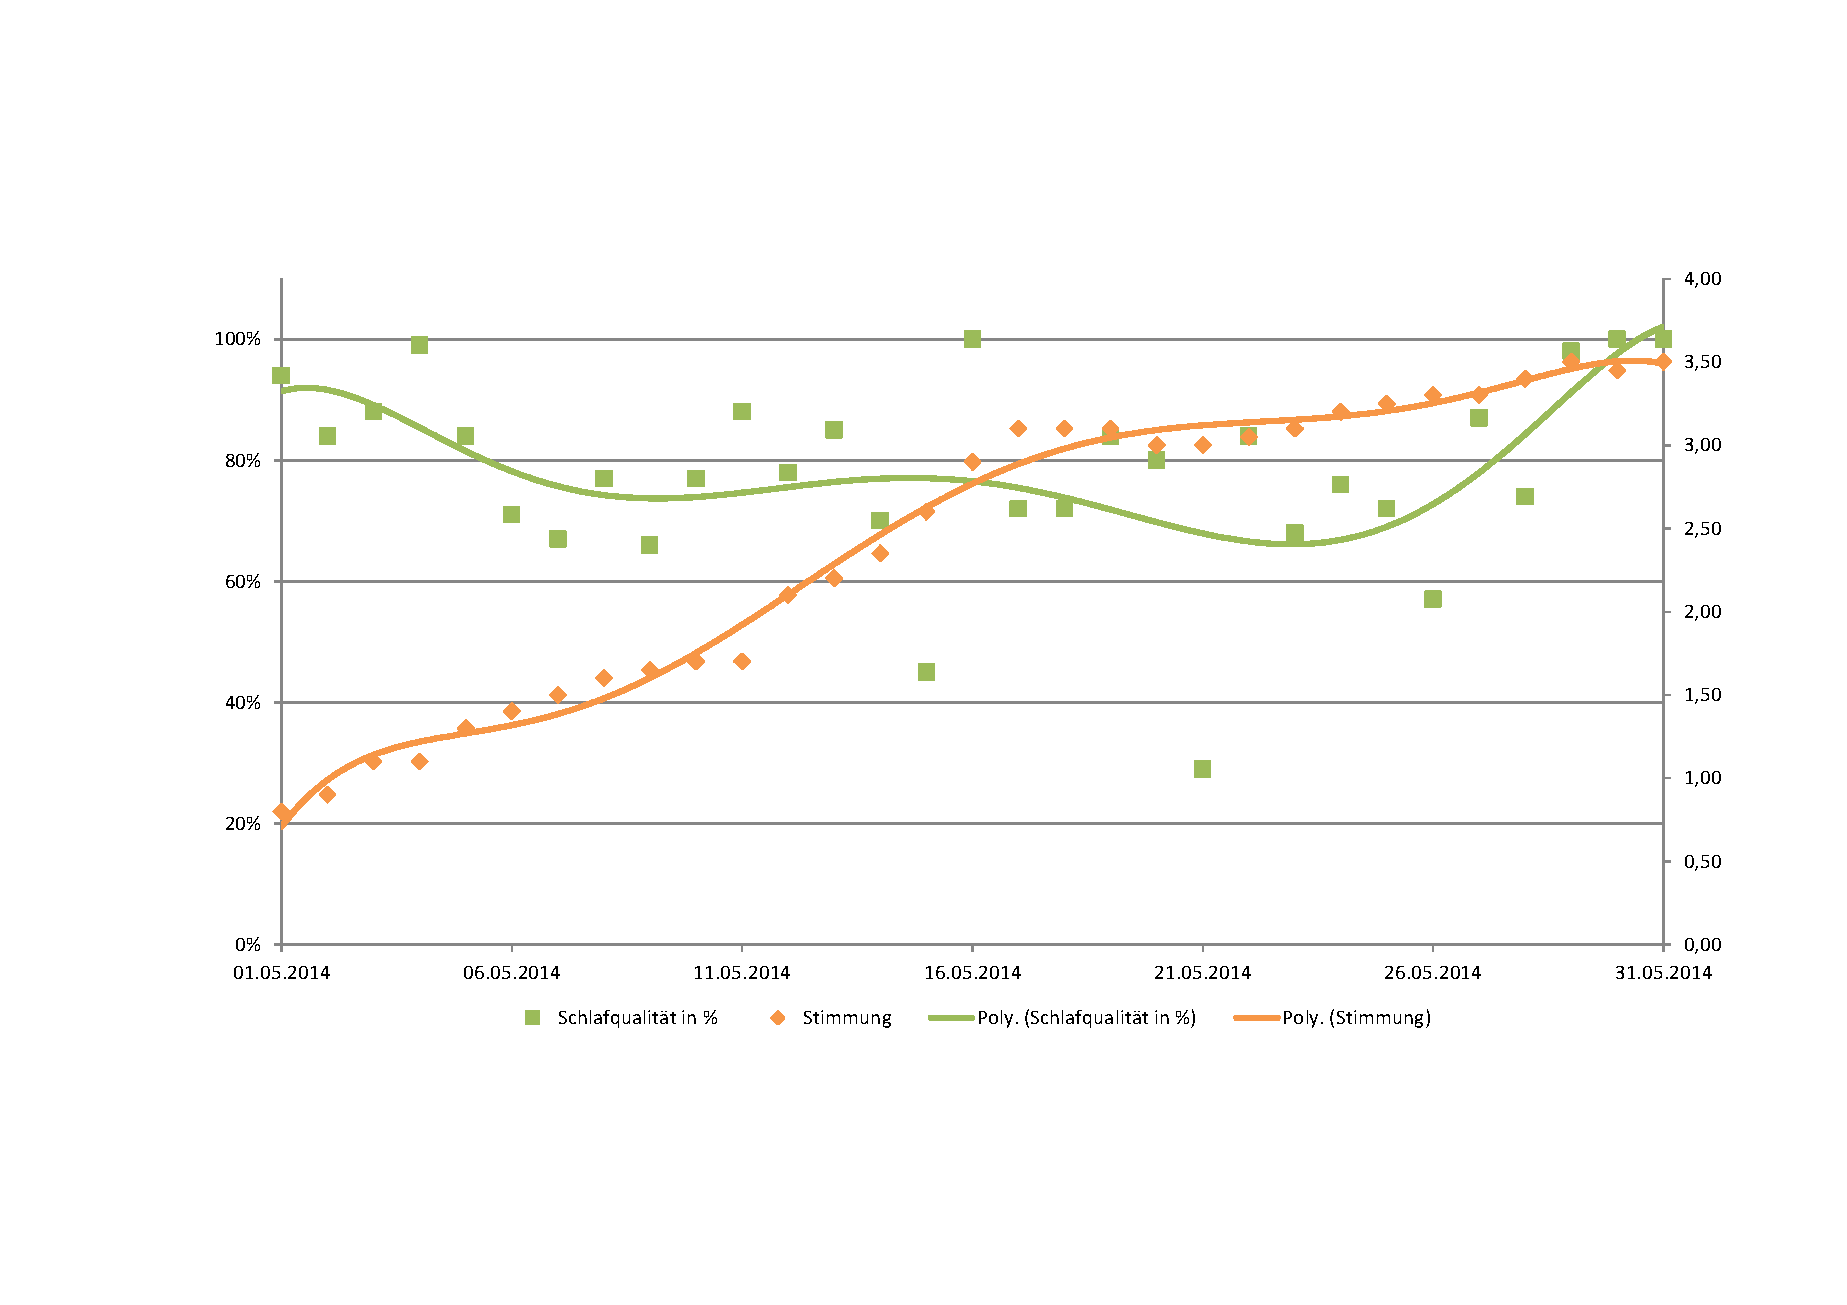
\includegraphics[angle=270,width=0.8\textwidth]{images/Analyse/Sleep-Mood} 
        \caption[Daten der Stimmung und der Schlafqualität]{Daten der Stimmung und der Schlafqualität}
        \label{fig:ZusammenhangVonStimmungUndSchlafqualität}
\end{figure}

%% ==============================
\section{Zusammenhang von Schlafqualität und Schritten am Tag}
%% ==============================
\label{ch:AnalyseUndEvaluierung:sec:KorrelationVonSchlafqualitätUndSchrittenAmTag}

\begin{figure}[H]
\centering
        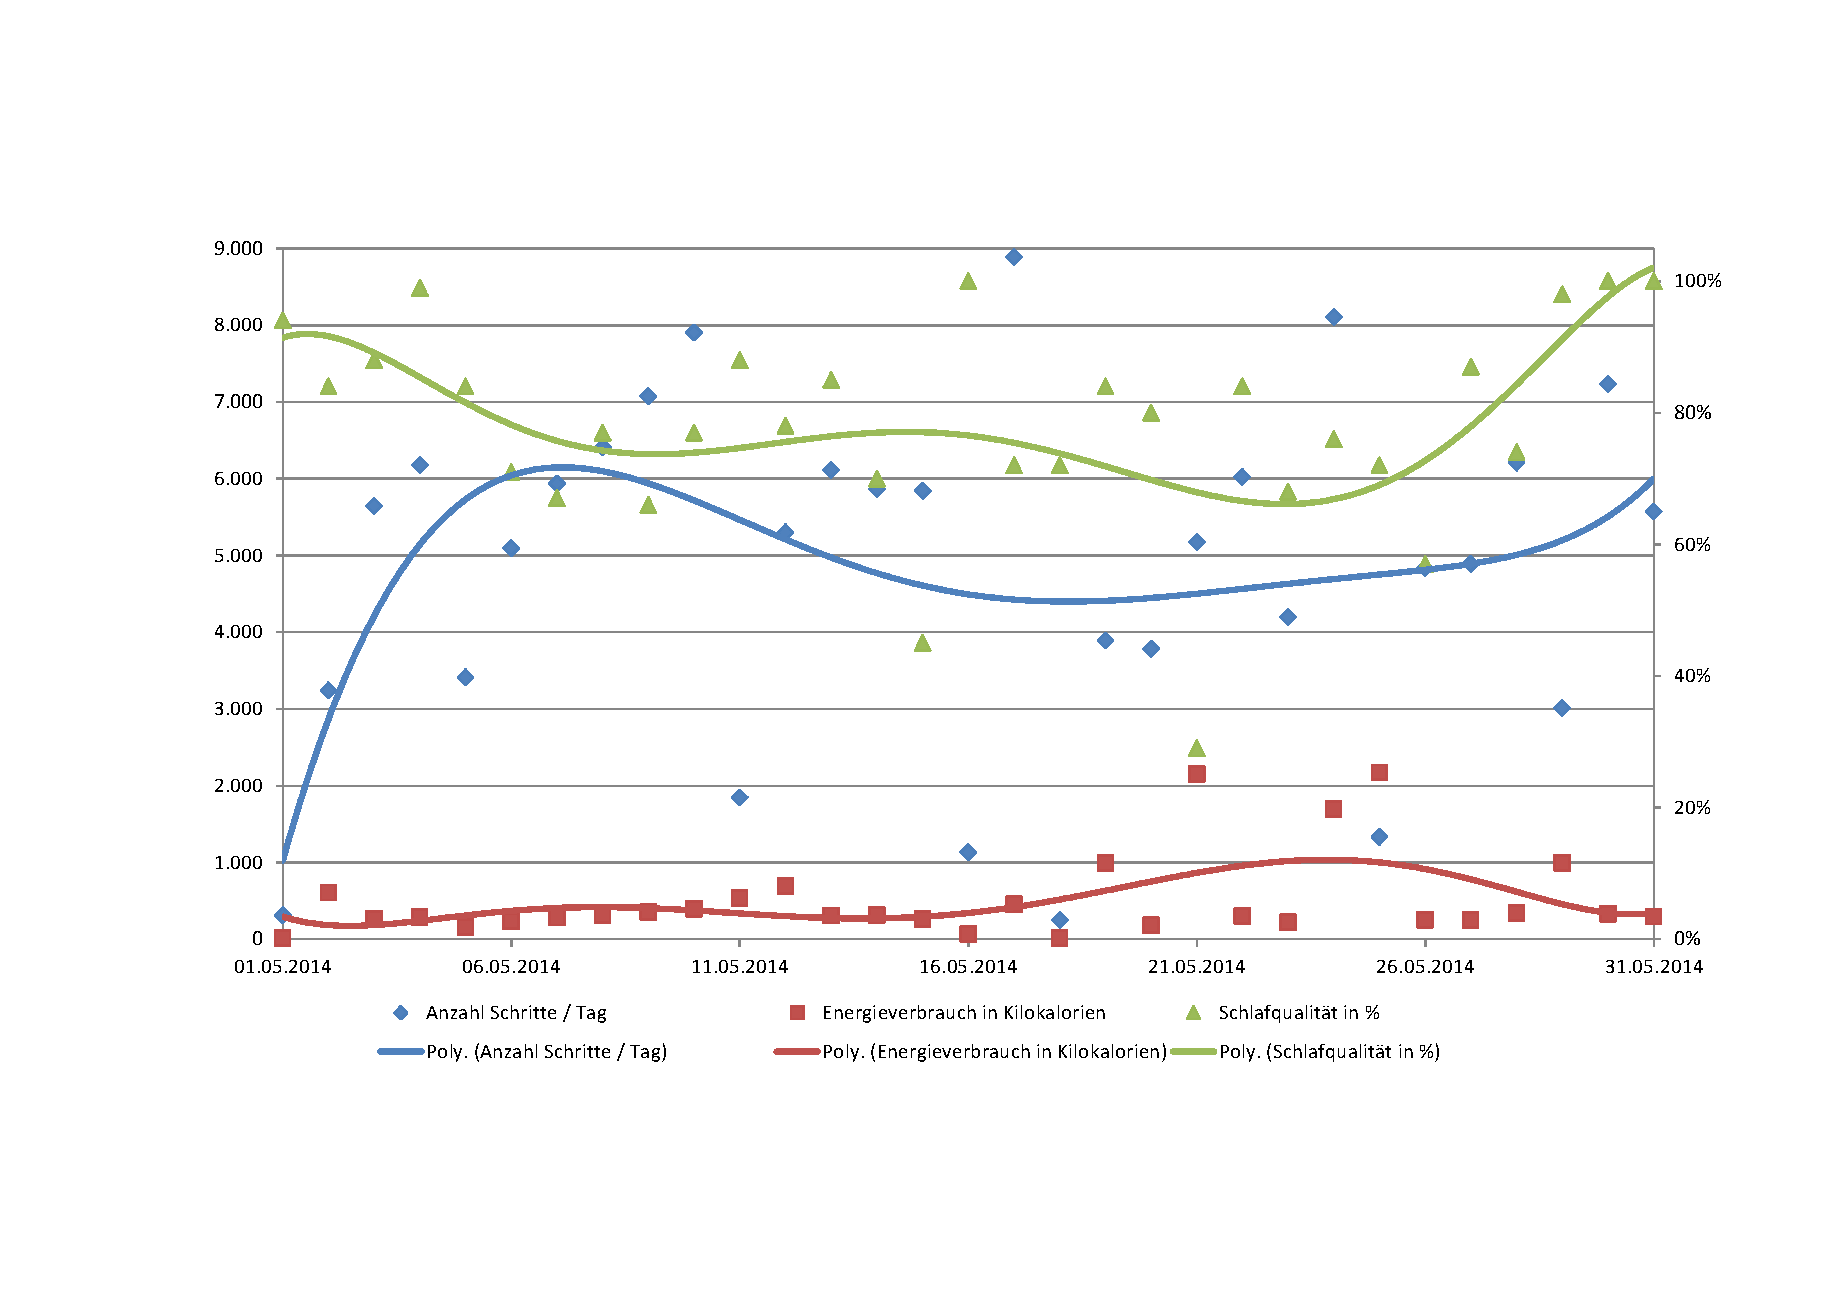
\includegraphics[angle=270,width=0.8\textwidth]{images/Analyse/Sleep-Steps-kcal} 
        \caption[Daten der Stimmung, der Schlafqualität und des Energieverbrauchs]{Daten der Stimmung, der Schlafqualität und des Energieverbrauchs}
        \label{fig:ZusammenhangVonSchlafqualitätSchrittenUndEnergieverbrauchAmTag}
\end{figure}

%% ==============================
\section{Zusammenfassung}
%% ==============================
\label{ch:Analyse:sec:zusammenfassung}


Diese Analyse liefert auf Basis einer ausführlichen Datenanalyse mit den gängigen Verfahren der Datenanalyse und -auswertung, der zuvor gewonnenen Daten, ein sehr exaktes Bild über die Zusammenhänge der jeweiligen Aktivitäten.
Die graphische Darstellung orientiert sich strikt an der Leitfrage des Projekts. 
Dadurch erhält der Leser eine erste Orientierung in welche Richtung die Beantwortung der Leitfrage ziehlen wird.

%% inferenzstatistik kann => nicht applyable weil nicht repräsentativ, referenzieren auf relativierung

%%% Local Variables: 
%%% mode: latex
%%% TeX-master: "thesis"
%%% End: 
     % Analyse
%% zusammenf.tex
%% $Id: zusammenf.tex 61 2012-05-03 13:58:03Z bless $
%%
% !TEX root = thesis.tex

\chapter{Zusammenfassung und Ausblick}
\label{ch:Zusammenfassung}
%% ==============================

Diese Analyse liefert auf Basis einer ausführlichen Datenanalyse mit den gängigen Verfahren der Datenanalyse und -auswertung, der zuvor gewonnenen Daten, ein sehr exaktes Bild über die Zusammenhänge der jeweiligen Aktivitäten.
Die graphische Darstellung orientiert sich strikt an der Leitfrage des Projekts. 
Dadurch erhält der Leser eine erste Orientierung in welche Richtung die Beantwortung der Leitfrage ziehlen wird.

Fazit:
Ob sich das Wohlbefinden durch Quantified Self verbessern lässt, kann man nicht durch Zahlen belegen. Es hängt von einem Selbst ab, inwiefern man sich damit besser fühlt.
*anregung motivation, interne konkurrenz(mehr laufen im projekt), ob es wirklich dazu beiträgt dass man gesünder ist ist eine andere frage, aber gefühlt fühlt man sich besser.
ziel von QS ist es nicht das leben zu verbessern, sonder dass man sich selbst besser fühlt. in sofern lässt sich die frage ob sich das wohlbefinden durch QS verbesern lässt mich ja beantworten.

%%% Local Variables: 
%%% mode: latex
%%% TeX-master: "thesis"
%%% End: 
   % Zusammenfassung und Ausblick

%% ++++++++++++++++++++++++++++++++++++++++++
%% Anhang
%% ++++++++++++++++++++++++++++++++++++++++++
\phantomsection
\appendix
%\include{
%\input{anhang_a}
%\input{anhang_b}

%% ++++++++++++++++++++++++++++++++++++++++++
%% Literatur
%% ++++++++++++++++++++++++++++++++++++++++++
%  mit dem Befehl \nocite werden auch nicht 
%  zitierte Referenzen abgedruckt
\cleardoublepage
\phantomsection
\addcontentsline{toc}{chapter}{\bibname}
% $ bibtex thesis
%%
%\nocite{*} % nur angeben, wenn auch nicht im Text zitierte Quellen 
           % erscheinen sollen
\bibliographystyle{ieeetr} % mit abgekÃŒrzten Vornamen der Autoren
%\bibliographystyle{gerplain} % abbrvnat unsrtnat
%\bibliographystyle{plainurl} % abbrvnat unsrtnat
% spezielle Zitierstile: Labels mit vier Buchstaben und Jahreszahl
%\bibliographystyle{itmalpha}  % ausgeschriebene Vornamen der Autoren
\bibliography{thesis}

\listoffigures
\listoftables
%% ++++++++++++++++++++++++++++++++++++++++++
%% Index
%% ++++++++++++++++++++++++++++++++++++++++++
\ifnotdraft{
\cleardoublepage
\phantomsection
%\printindex            % Index, Stichwortverzeichnis
}
\end{document}
%% end of file
